\documentclass[11pt, a4paper]{article}
\usepackage[utf8]{inputenc}
\usepackage{geometry}
\usepackage{graphicx}
\usepackage{amsmath}
\usepackage{booktabs}
\usepackage{float}
\usepackage{listings}
\usepackage{xcolor}
\usepackage[hidelinks]{hyperref}
\usepackage{array}
\usepackage{subcaption}
\usepackage{xurl}
\usepackage{tikz}

\hypersetup{
    colorlinks=true,
    urlcolor=blue,
    linkcolor=black,
    citecolor=black
}

% ==========================================
% GROUP DETAILS - fill these in before submitting
% (names seen in the git history: Jaindu Samaranayaka, Kaveesha, Thiviru Malitha,
%  Hasindu Wanigasundara - check spelling and add index numbers)
% ==========================================
\newcommand{\GroupNo}{XX}
\newcommand{\MemberOne}{230680M -- W.M.H. Wanigasundara}
\newcommand{\MemberTwo}{Index No. -- Name}
\newcommand{\MemberThree}{Index No. -- Name}
\newcommand{\MemberFour}{Index No. -- Name}
\newcommand{\RepoURL}{https://github.com/jaindusamaranayaka/EN3150-ConvNets-Image-Classifier}

% --- Page Header & Footer Setup ---
\usepackage{fancyhdr}
\pagestyle{fancy}
\fancyhf{} % Clear default headers and footers

% Header setup
\lhead{\small Assignment 03}
\rhead{\small EN3150 Pattern Recognition}

% Footer setup
\lfoot{\small Group \GroupNo}
\rfoot{\small Page \thepage}

% Line formatting
\renewcommand{\headrulewidth}{0.4pt}
\renewcommand{\footrulewidth}{0.4pt}

\geometry{top=1in, bottom=1in, left=0.8in, right=0.8in}

% --- Code Listing Formatting ---
\definecolor{codegreen}{rgb}{0,0.6,0}
\definecolor{codegray}{rgb}{0.5,0.5,0.5}
\definecolor{codepurple}{rgb}{0.58,0,0.82}
\definecolor{backcolour}{rgb}{0.95,0.95,0.92}

\lstdefinestyle{mystyle}{
    backgroundcolor=\color{backcolour},
    commentstyle=\color{codegreen},
    keywordstyle=\color{magenta},
    numberstyle=\tiny\color{codegray},
    stringstyle=\color{codepurple},
    basicstyle=\ttfamily\footnotesize,
    breakatwhitespace=false,
    breaklines=true,
    captionpos=b,
    keepspaces=true,
    numbers=left,
    numbersep=5pt,
    showspaces=false,
    showstringspaces=false,
    showtabs=false,
    tabsize=2
}

\lstset{style=mystyle}

\begin{document}
\setlength{\headwidth}{\textwidth}
% ==========================================
% COVER PAGE
% ==========================================
\begin{titlepage}
\begin{tikzpicture}[remember picture, overlay]
    \draw[thick] ([xshift=1cm, yshift=-1cm]current page.north west) rectangle ([xshift=-1cm, yshift=1cm]current page.south east);
\end{tikzpicture}
    \begin{center}
        \vspace*{1cm}

        \textbf{\Large UNIVERSITY OF MORATUWA}

        \vspace{0.5cm}
        DEPARTMENT OF ELECTRONIC \& TELECOMMUNICATION ENGINEERING

        \vspace{1.5cm}

        
\includegraphics[width=0.4\textwidth]{Mora_Sysmbol.png}

        \vspace{1.5cm}

        \textbf{\Huge Assignment 03}

        \vspace{0.5cm}

        \textbf{\Large EN3150 Pattern Recognition}\\[0.4cm]\textbf{\large Resource-Constrained CNN for Edge Image Classification}

        \vspace{1.5cm}

        \textbf{\Large Group \GroupNo}

        \vspace{0.6cm}

        \begin{tabular}{l}
            \MemberOne \\[0.15cm]
            \MemberTwo \\[0.15cm]
            \MemberThree \\[0.15cm]
            \MemberFour
        \end{tabular}

        \vspace{1cm}

        \small GitHub: \url{\RepoURL}

        \vspace{0.5cm}

        \textbf{Date: \today}

    \end{center}
\end{titlepage}

\newpage
\setcounter{page}{1}

\tableofcontents

\newpage

% ==========================================
\section{Introduction}
% ==========================================

This report designs, trains and compares image classifiers for a resource-constrained edge device such as a
microcontroller or a Raspberry Pi. Two custom convolutional neural networks (CNNs) were built from scratch: a standard
CNN (\textbf{Model A}) and a lightweight CNN based on depthwise separable convolutions (\textbf{Model B}, under
100,000 parameters). They are compared with two ImageNet-pretrained lightweight networks, \textbf{MobileNetV2} and
\textbf{EfficientNet-B0}, fine-tuned on the same data. All models classify $64 \times 64$ traffic-sign images into 43
classes and are evaluated on accuracy, memory footprint and computational cost.

All models were implemented in Python with PyTorch, trained on the same data splits with the same augmentation, and
timed on the same machine (NVIDIA GTX 1660 Ti GPU). The code, notebooks and every result file are in the GitHub
repository: \url{\RepoURL}.

% ==========================================
\section{Dataset and Data Preparation}
% ==========================================

\subsection{Dataset}

The \textbf{German Traffic Sign Recognition Benchmark (GTSRB)} \cite{gtsrb} was used. It contains real-world
photographs of 43 traffic-sign classes (speed limits, warnings, prohibitions and mandatory signs) under varying
lighting, blur, partial occlusion and viewing angle. The original images range from about $15 \times 15$ to
$250 \times 250$ pixels, so the dataset is naturally low resolution, which suits an edge-sensor scenario. The GTSRB
training set (26,640 images, loaded through \texttt{torchvision}) was used and split into training, validation and
test sets as required by the assignment.

\subsection{Pre-processing}

\begin{itemize}
    \item \textbf{Resolution:} every image is resized to $64 \times 64 \times 3$, the maximum resolution allowed, to
          emulate a low-resource camera (Figure~\ref{fig:samples}).
    \item \textbf{Normalisation:} pixel values are scaled to $[-1, 1]$ for the custom models. The pretrained models use
          the ImageNet mean and standard deviation, which their weights expect.
    \item \textbf{Augmentation (training set only):} random brightness and contrast ($\pm 20\%$), rotation
          ($\pm 8^\circ$), translation ($\pm 5\%$) and scaling (0.95--1.05). Horizontal flips are deliberately
          \emph{not} used, because flipping changes the meaning of some signs (e.g.\ ``turn left'' becomes ``turn right'').
\end{itemize}

\subsection{Data Split}

The images were split once, randomly with a fixed seed (42), and the split was saved to CSV files so that
\emph{every} model is trained and tested on exactly the same images (Table~\ref{tab:split}). The three sets are
disjoint and all 43 classes appear in each. The classes are imbalanced, from 150 to 1,500 images per class
(Figure~\ref{fig:classes}); macro-averaged precision and recall are therefore reported alongside accuracy, so that
rare classes count as much as common ones.

\begin{table}[H]
\centering
\caption{Data split (seed 42).}
\label{tab:split}
\begin{tabular}{lrr}
\toprule
\textbf{Set} & \textbf{Images} & \textbf{Share} \\
\midrule
Training   & 18,648 & 70\% \\
Validation & 3,996  & 15\% \\
Test       & 3,996  & 15\% \\
\midrule
Total      & 26,640 & 100\% \\
\bottomrule
\end{tabular}
\end{table}

\begin{figure}[H]
\centering
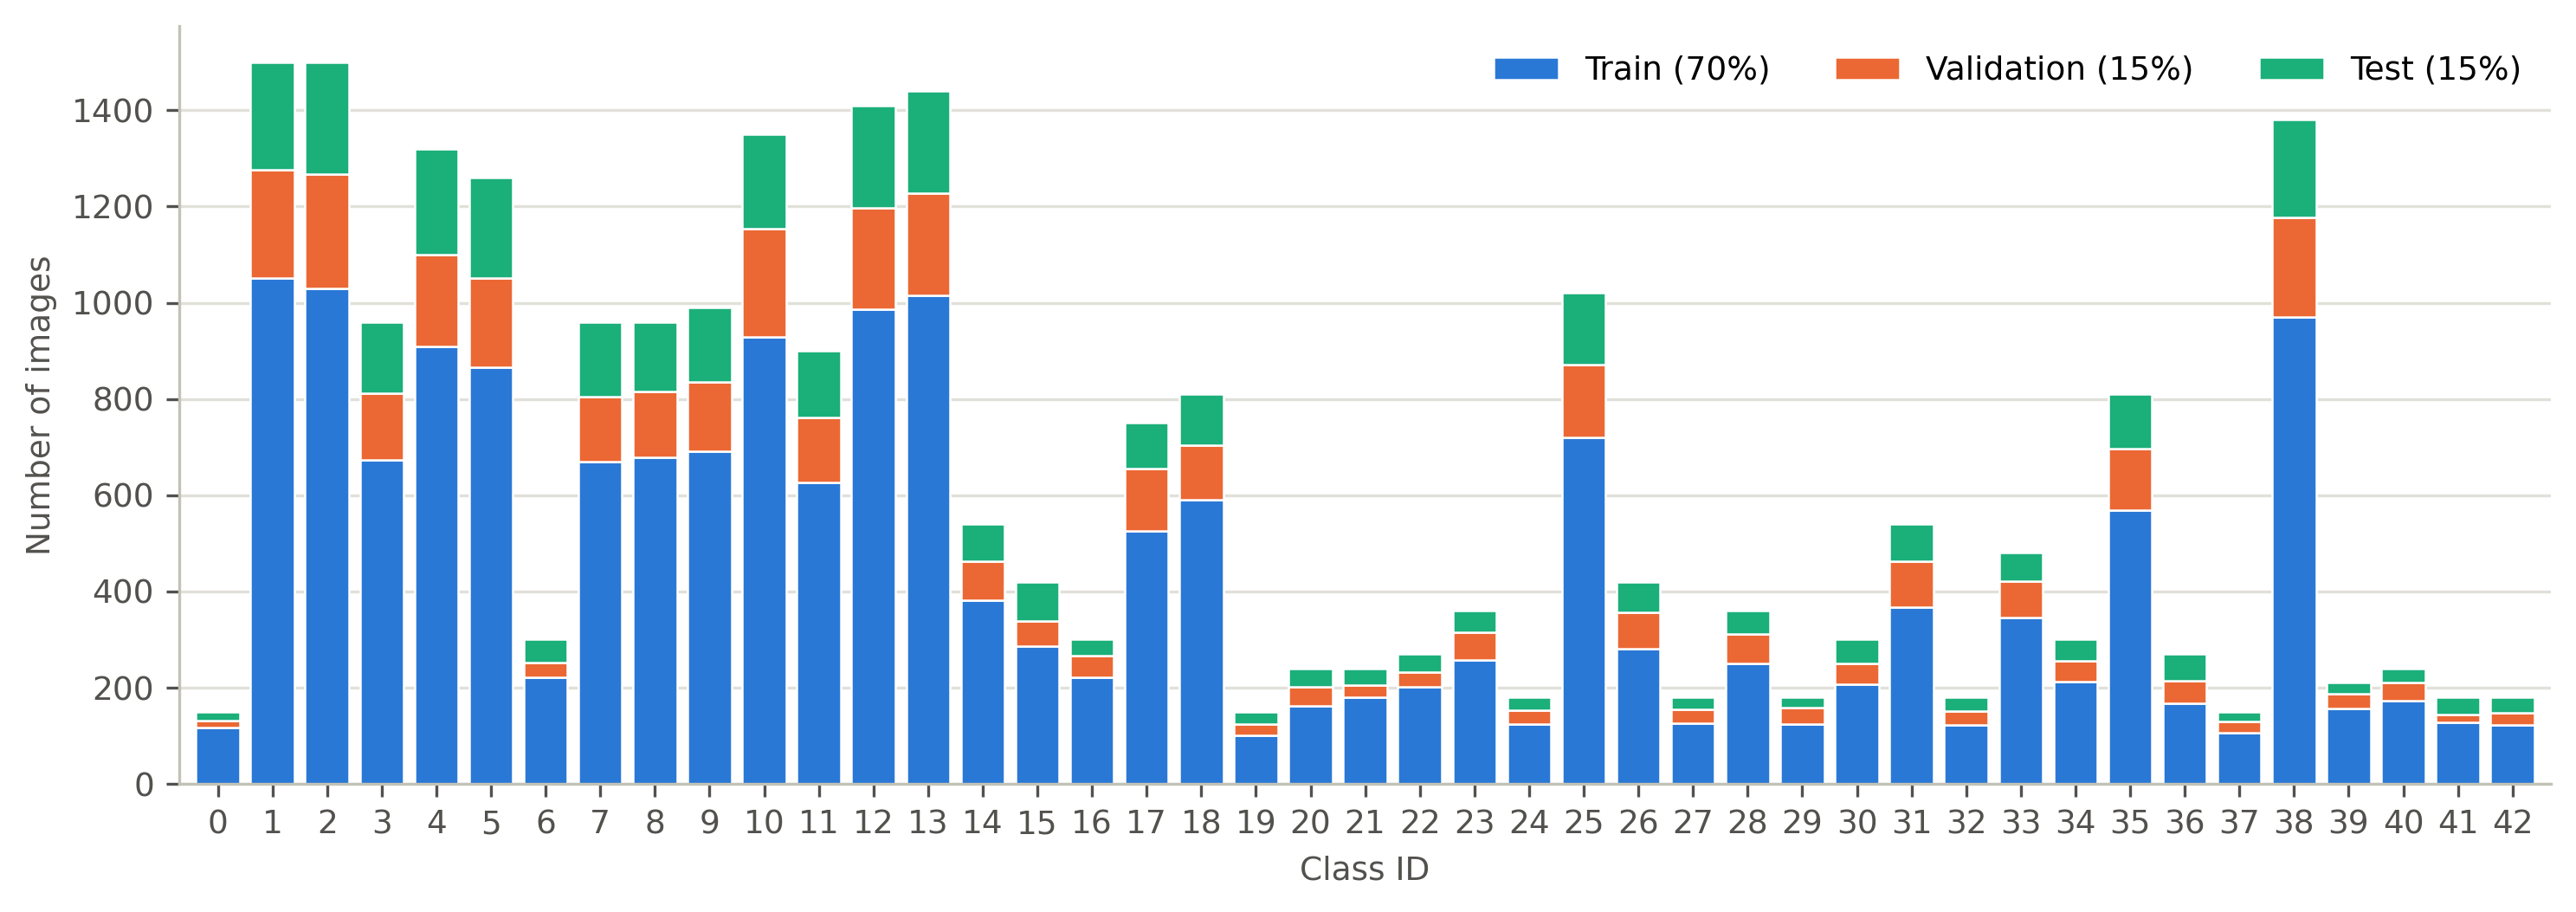
\includegraphics[width=\textwidth]{figures/class_distribution.png}
\caption{Number of images per class in each split. Every class keeps roughly the 70/15/15 proportion.}
\label{fig:classes}
\end{figure}

\begin{figure}[H]
\centering
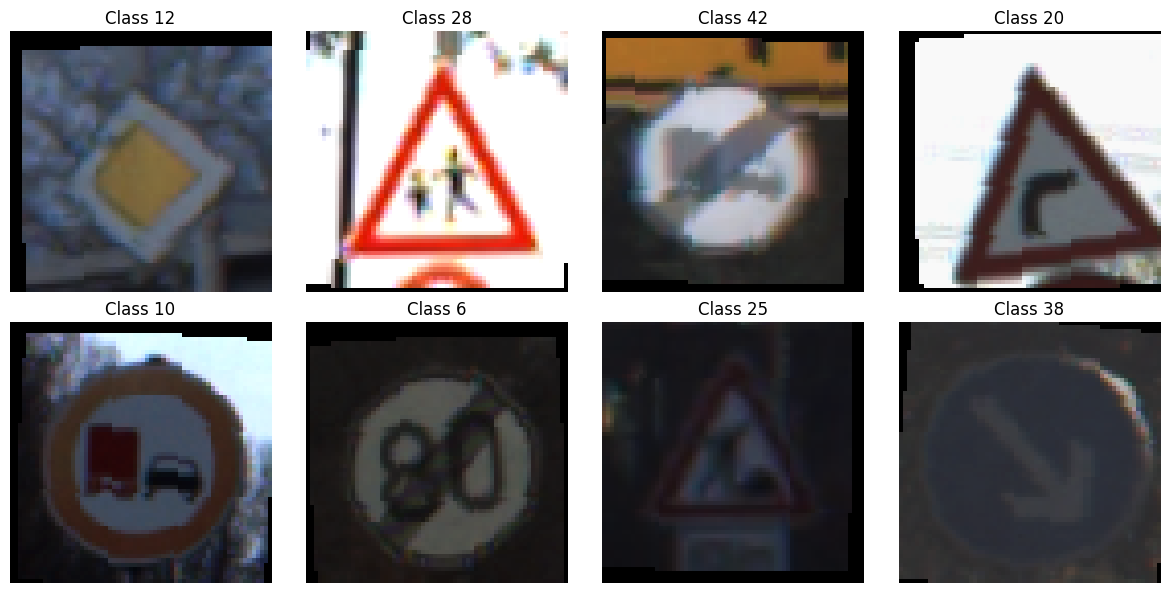
\includegraphics[width=0.75\textwidth]{figures/sample_images.png}
\caption{Training images after resizing to $64 \times 64$ and augmentation (black corners come from the random rotation).}
\label{fig:samples}
\end{figure}

% ==========================================
\section{Custom Architecture Design}
% ==========================================

Both custom models use the same four-stage layout so that they differ \emph{only} in the type of convolution. Each
stage halves the spatial resolution with $2 \times 2$ max-pooling while the channels grow
$3 \rightarrow 16 \rightarrow 32 \rightarrow 32 \rightarrow 32$, giving a $32 \times 4 \times 4 = 512$-value feature
vector that a single fully connected layer maps to the 43 class scores. The layer widths were kept small on purpose:
with only four pooling stages and 32 final channels, the classifier stays at 22,059 parameters.

\subsection{Model A: Standard CNN}

Model A interleaves standard $3 \times 3$ convolutions (stride 1, padding 1) with ReLU and $2 \times 2$ max-pooling
(stride 2). A standard convolution with kernel size $k$, $C_{in}$ input and $C_{out}$ output channels has
\begin{equation}
    P_{\text{conv}} = k^2 \, C_{in} \, C_{out} + C_{out}
\end{equation}
trainable parameters, and costs $H \cdot W \cdot k^2 \, C_{in} \, C_{out}$ multiply--accumulate operations (MACs) on an
$H \times W$ output. Table~\ref{tab:modelA} details every layer.

\begin{table}[H]
\centering
\caption{Model A (standard CNN). Parameters and MACs per $64 \times 64$ image.}
\label{tab:modelA}
\resizebox{\textwidth}{!}{%
\begin{tabular}{llllrr}
\toprule
\textbf{Layer} & \textbf{Kernel} & \textbf{Filters / units} & \textbf{Output} & \textbf{Parameters} & \textbf{MACs} \\
\midrule
Input            & --           & --  & $3 \times 64 \times 64$  & -- & -- \\
Conv2d + ReLU    & $3 \times 3$ & 16  & $16 \times 64 \times 64$ & $27 \cdot 16 + 16 = 448$ & 1,769,472 \\
MaxPool          & $2 \times 2$ & --  & $16 \times 32 \times 32$ & 0 & -- \\
Conv2d + ReLU    & $3 \times 3$ & 32  & $32 \times 32 \times 32$ & $144 \cdot 32 + 32 = 4{,}640$ & 4,718,592 \\
MaxPool          & $2 \times 2$ & --  & $32 \times 16 \times 16$ & 0 & -- \\
Conv2d + ReLU    & $3 \times 3$ & 32  & $32 \times 16 \times 16$ & $288 \cdot 32 + 32 = 9{,}248$ & 2,359,296 \\
MaxPool          & $2 \times 2$ & --  & $32 \times 8 \times 8$   & 0 & -- \\
Conv2d + ReLU    & $3 \times 3$ & 32  & $32 \times 8 \times 8$   & 9,248 & 589,824 \\
MaxPool          & $2 \times 2$ & --  & $32 \times 4 \times 4$   & 0 & -- \\
Flatten          & --           & --  & 512                      & 0 & -- \\
Fully connected  & --           & 43  & 43                       & $512 \cdot 43 + 43 = 22{,}059$ & 22,016 \\
\midrule
\textbf{Total}   & & & & \textbf{45,643} & \textbf{9,459,200} \\
\bottomrule
\end{tabular}}
\end{table}

\subsection{Model B: Lightweight CNN with Depthwise Separable Convolutions}

Model B replaces each standard convolution with a \textbf{depthwise separable convolution} \cite{mobilenetv1}, which
splits the operation into two cheaper steps:
\begin{enumerate}
    \item a \textbf{depthwise} $3 \times 3$ convolution that filters each input channel separately
          (\texttt{groups = $C_{in}$}, no bias, since the next layer adds one), and
    \item a \textbf{pointwise} $1 \times 1$ convolution that mixes the channels and produces $C_{out}$ outputs,
\end{enumerate}
followed by ReLU and the same max-pooling. Its parameter count and cost are
\begin{equation}
    P_{\text{DS}} = k^2 \, C_{in} + C_{in} \, C_{out} + C_{out}, \qquad
    \text{MACs}_{\text{DS}} = H \cdot W \cdot (k^2 \, C_{in} + C_{in} \, C_{out}),
\end{equation}
so the cost relative to a standard convolution is $\frac{1}{C_{out}} + \frac{1}{k^2}$, about $\frac{1}{32} + \frac{1}{9}
\approx 0.14$ for the $32 \to 32$ layers. Table~\ref{tab:modelB} details every layer.

\begin{table}[H]
\centering
\caption{Model B (depthwise separable CNN). Max-pooling, flatten and output shapes are identical to Model A.}
\label{tab:modelB}
\begin{tabular}{lrrrrr}
\toprule
\textbf{Block} & \textbf{Depthwise $3 \times 3$} & \textbf{Pointwise $1 \times 1$} & \textbf{Parameters} & \textbf{MACs} & \textbf{Model A} \\
               & $k^2 C_{in}$ & $C_{in} C_{out} + C_{out}$ & & & \textbf{params} \\
\midrule
$3 \rightarrow 16$   & 27  & 64    & 91     & 307,200   & 448 \\
$16 \rightarrow 32$  & 144 & 544   & 688    & 671,744   & 4,640 \\
$32 \rightarrow 32$  & 288 & 1,056 & 1,344  & 335,872   & 9,248 \\
$32 \rightarrow 32$  & 288 & 1,056 & 1,344  & 83,968    & 9,248 \\
FC $512 \rightarrow 43$ & -- & -- & 22,059 & 22,016    & 22,059 \\
\midrule
\textbf{Total} & & & \textbf{25,526} & \textbf{1,420,800} & \textbf{45,643} \\
\bottomrule
\end{tabular}
\end{table}

Model B has \textbf{25,526} trainable parameters, well below the 100,000 limit, and needs \textbf{85\% fewer MACs}
than Model A (1.42\,M vs 9.46\,M). The convolutional layers shrink from 23,584 to 3,467 parameters, so the fully
connected layer now holds 86\% of Model B's parameters; any further reduction would have to target the classifier
(e.g.\ global average pooling instead of flattening).

\subsection{Hardware-Aware Choice of Activation Function}

\textbf{ReLU}, $f(x) = \max(0, x)$, is used after every convolution in both models:
\begin{itemize}
    \item \textbf{No transcendental functions.} ReLU is a single comparison per value. Sigmoid and tanh need an
          exponential for every activation, which is slow on microcontrollers without a floating-point unit and
          typically needs lookup tables or polynomial approximations.
    \item \textbf{Quantisation friendly.} ReLU is piecewise linear and works directly in 8-bit integer arithmetic,
          the usual format for deploying models on edge hardware.
    \item \textbf{Sparse activations.} Negative inputs become exactly zero, which reduces the work in later layers on
          hardware that skips zeros.
    \item \textbf{Max-pooling} likewise needs only comparisons, and \textbf{softmax is not needed at inference}: the
          predicted class is the arg-max of the logits, so the exponentials of softmax are only used inside the
          cross-entropy loss during training.
\end{itemize}

% ==========================================
\section{Optimizer Selection and Tuning}
% ==========================================

\subsection{Experimental Set-up}

The optimizer study was run as a controlled experiment on Model A: every run starts from the \emph{same} saved random
initialisation, sees mini-batches in the same order, and trains for 20 epochs with batch size 32 and cross-entropy
loss. Only the optimizer changes. In addition to the three required optimizers, a momentum sweep
($\beta \in \{0, 0.5, 0.9, 0.99\}$) and a control run (plain SGD with $\eta = 0.1$) were added to explain the effect of
momentum. Each run is tested with its final-epoch weights.

\begin{table}[H]
\centering
\caption{Optimizer comparison on Model A (20 epochs).}
\label{tab:optim}
\resizebox{\textwidth}{!}{%
\begin{tabular}{lrrrrrr}
\toprule
\textbf{Optimizer} & \textbf{Epochs to} & \textbf{Final train} & \textbf{Best val} & \textbf{Test} & \textbf{Test} & \textbf{Batch-loss} \\
                   & \textbf{95\% val} & \textbf{loss} & \textbf{acc (\%)} & \textbf{acc (\%)} & \textbf{recall (\%)} & \textbf{std} \\
\midrule
SGD ($\eta = 0.01$)                          & 14    & 0.092 & 97.27 & 97.10 & 97.66 & 0.085 \\
SGD + Momentum ($\eta = 0.01$, $\beta = 0.9$)  & 5     & 0.229 & 98.12 & 94.92 & 93.72 & 0.244 \\
\textbf{Adam ($\eta = 0.001$)}               & \textbf{4} & \textbf{0.031} & \textbf{98.92} & \textbf{98.15} & 97.48 & \textbf{0.056} \\
\midrule
SGD + Momentum ($\beta = 0.5$)               & 8     & 0.040 & 98.25 & 95.62 & 96.48 & 0.063 \\
SGD + Momentum ($\beta = 0.99$)              & never & 3.508 & 14.76 & 5.83  & 2.33  & 0.124 \\
SGD ($\eta = 0.1$, control)                  & 4     & 0.200 & 98.37 & 96.60 & 96.72 & 0.248 \\
\bottomrule
\end{tabular}}
\end{table}

\begin{figure}[H]
\centering
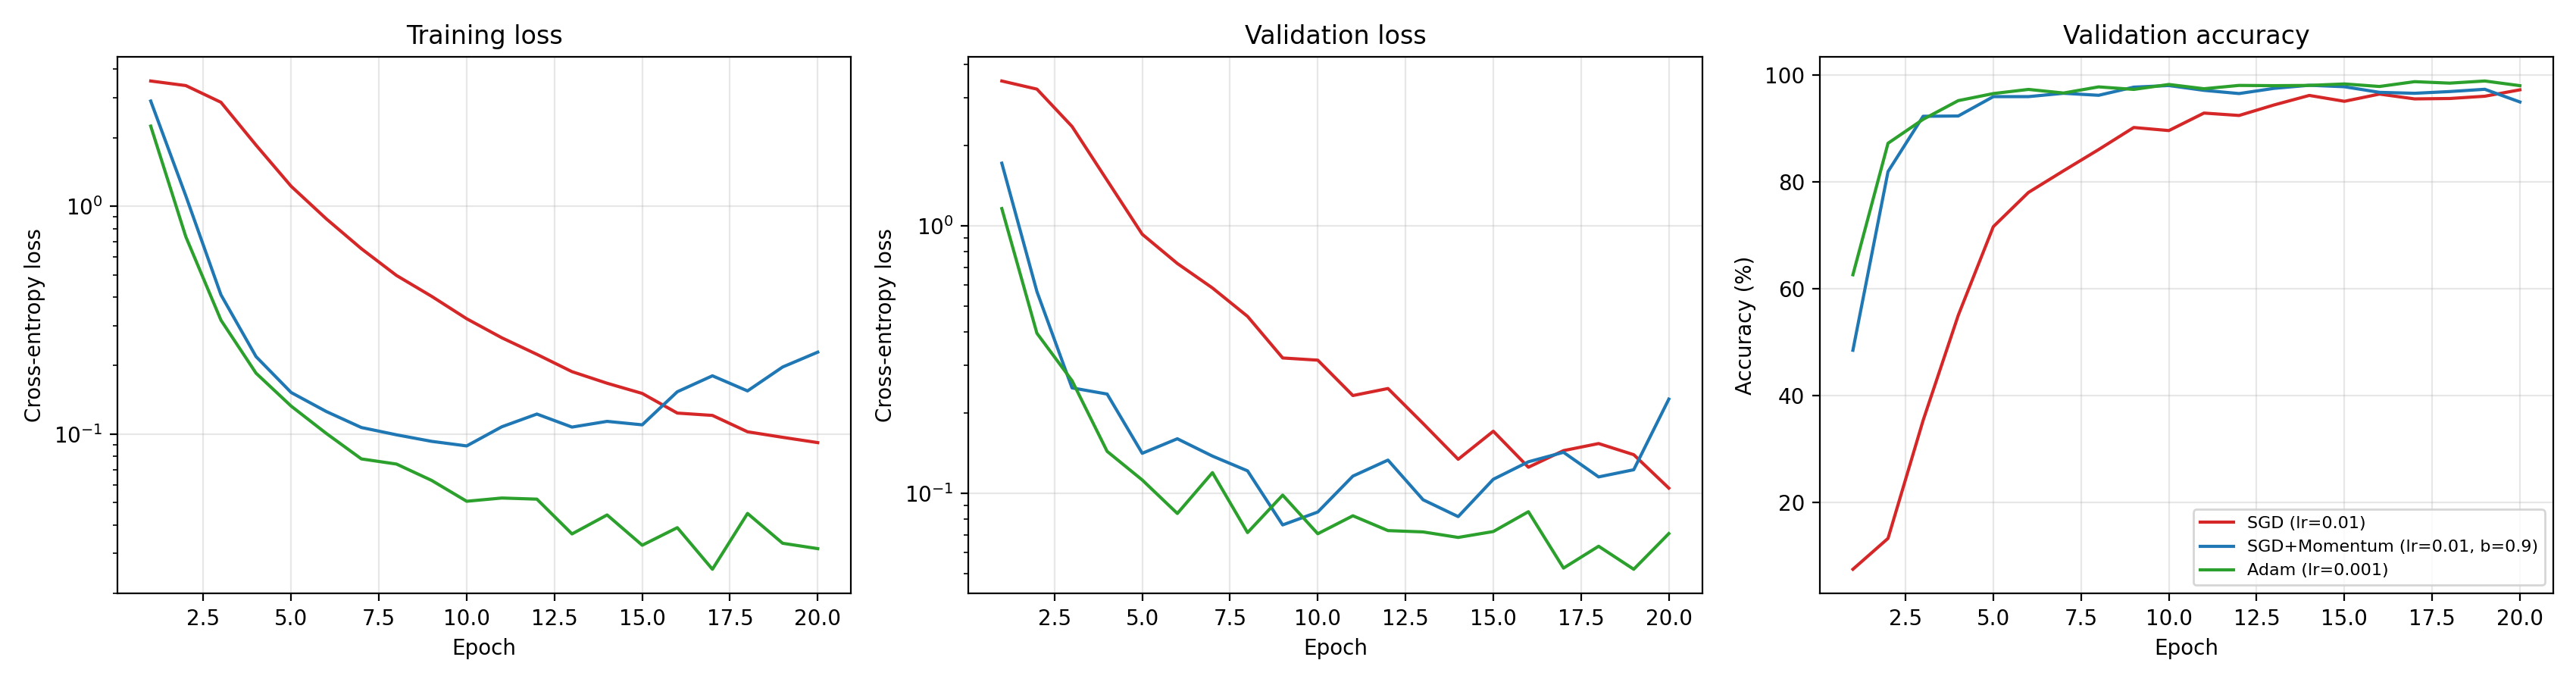
\includegraphics[width=\textwidth]{figures/optimizer_convergence.png}
\caption{Training loss, validation loss (log scale) and validation accuracy for SGD, SGD + Momentum and Adam.}
\label{fig:optim}
\end{figure}

\subsection{Selected Optimizer: Adam, $\eta = 0.001$}

\textbf{Adam} \cite{adam} with the standard learning rate $\eta = 0.001$ ($\beta_1 = 0.9$, $\beta_2 = 0.999$) was
selected for Models A and B (Figure~\ref{fig:optim}):
\begin{itemize}
    \item \textbf{Fastest convergence:} 95\% validation accuracy after 4 epochs, compared with 5 for SGD + Momentum and
          14 for plain SGD.
    \item \textbf{Best and most stable result:} the highest validation (98.92\%) and test (98.15\%) accuracy, the lowest
          final training loss (0.031) and the smoothest mini-batch loss in the last epoch (standard deviation 0.056).
    \item \textbf{No tuning required:} Adam adapts the step size of each parameter using running estimates of the mean
          and variance of its gradient, so the default $\eta = 0.001$ works without a learning-rate search. The SGD
          variants depend strongly on the hand-picked $\eta$ and $\beta$, as Table~\ref{tab:optim} shows.
\end{itemize}

\textbf{Plain SGD} is stable but slow: during the first two epochs its loss barely moves from the value of random
guessing ($\ln 43 \approx 3.76$), validation accuracy is only 71.6\% after 5 epochs, and 95\% is reached only at
epoch 14. It finishes close to Adam (97.10\% test) precisely because it never becomes unstable.

\subsection{Impact of the Momentum Parameter}

SGD with momentum keeps a decaying sum of past gradients, $v_{t} = \beta v_{t-1} + \nabla L$, and updates the weights
with $w_{t+1} = w_t - \eta v_t$. Directions in which the gradient is consistent accumulate speed, while oscillating
directions partly cancel. Figure~\ref{fig:momentum} and Table~\ref{tab:optim} show the effect of $\beta$:

\begin{itemize}
    \item \textbf{Faster convergence with larger $\beta$:} 14, 8 and 5 epochs to reach 95\% validation accuracy for
          $\beta = 0$, 0.5 and 0.9.
    \item \textbf{Overshooting when $\beta$ is too large:} with $\beta = 0.9$ the training loss is lowest at epoch 10
          (0.089) and then rises to 0.229 by epoch 20, and the mini-batch loss is the noisiest of all runs
          (std 0.244). Its final weights are therefore worse than its best epoch (94.92\% test vs 98.12\% best validation).
          With $\beta = 0.99$ the velocity grows so large that training becomes unstable in the first epochs and never
          recovers: the loss stays near 3.5, close to random guessing.
    \item \textbf{Momentum mostly acts as a larger effective step.} With momentum the effective step size is about
          $\eta / (1 - \beta)$, i.e.\ $0.01 / 0.1 = 0.1$ for $\beta = 0.9$. The control run, plain SGD with
          $\eta = 0.1$, behaves almost identically: 95\% at epoch 4 (vs 5), similar late-training noise (std 0.248 vs
          0.244) and the same late rise in training loss. Much of momentum's speed-up therefore comes from taking larger
          effective steps, not only from smoothing the gradient direction.
\end{itemize}

Getting momentum's early speed without the late instability would need a moderate $\beta$ combined with a decaying
learning rate. Adam provides fast and stable convergence without this tuning, which is why it was chosen. A
preliminary three-optimizer run on Model B (batch size 128) also ranked Adam first.

\begin{figure}[H]
\centering
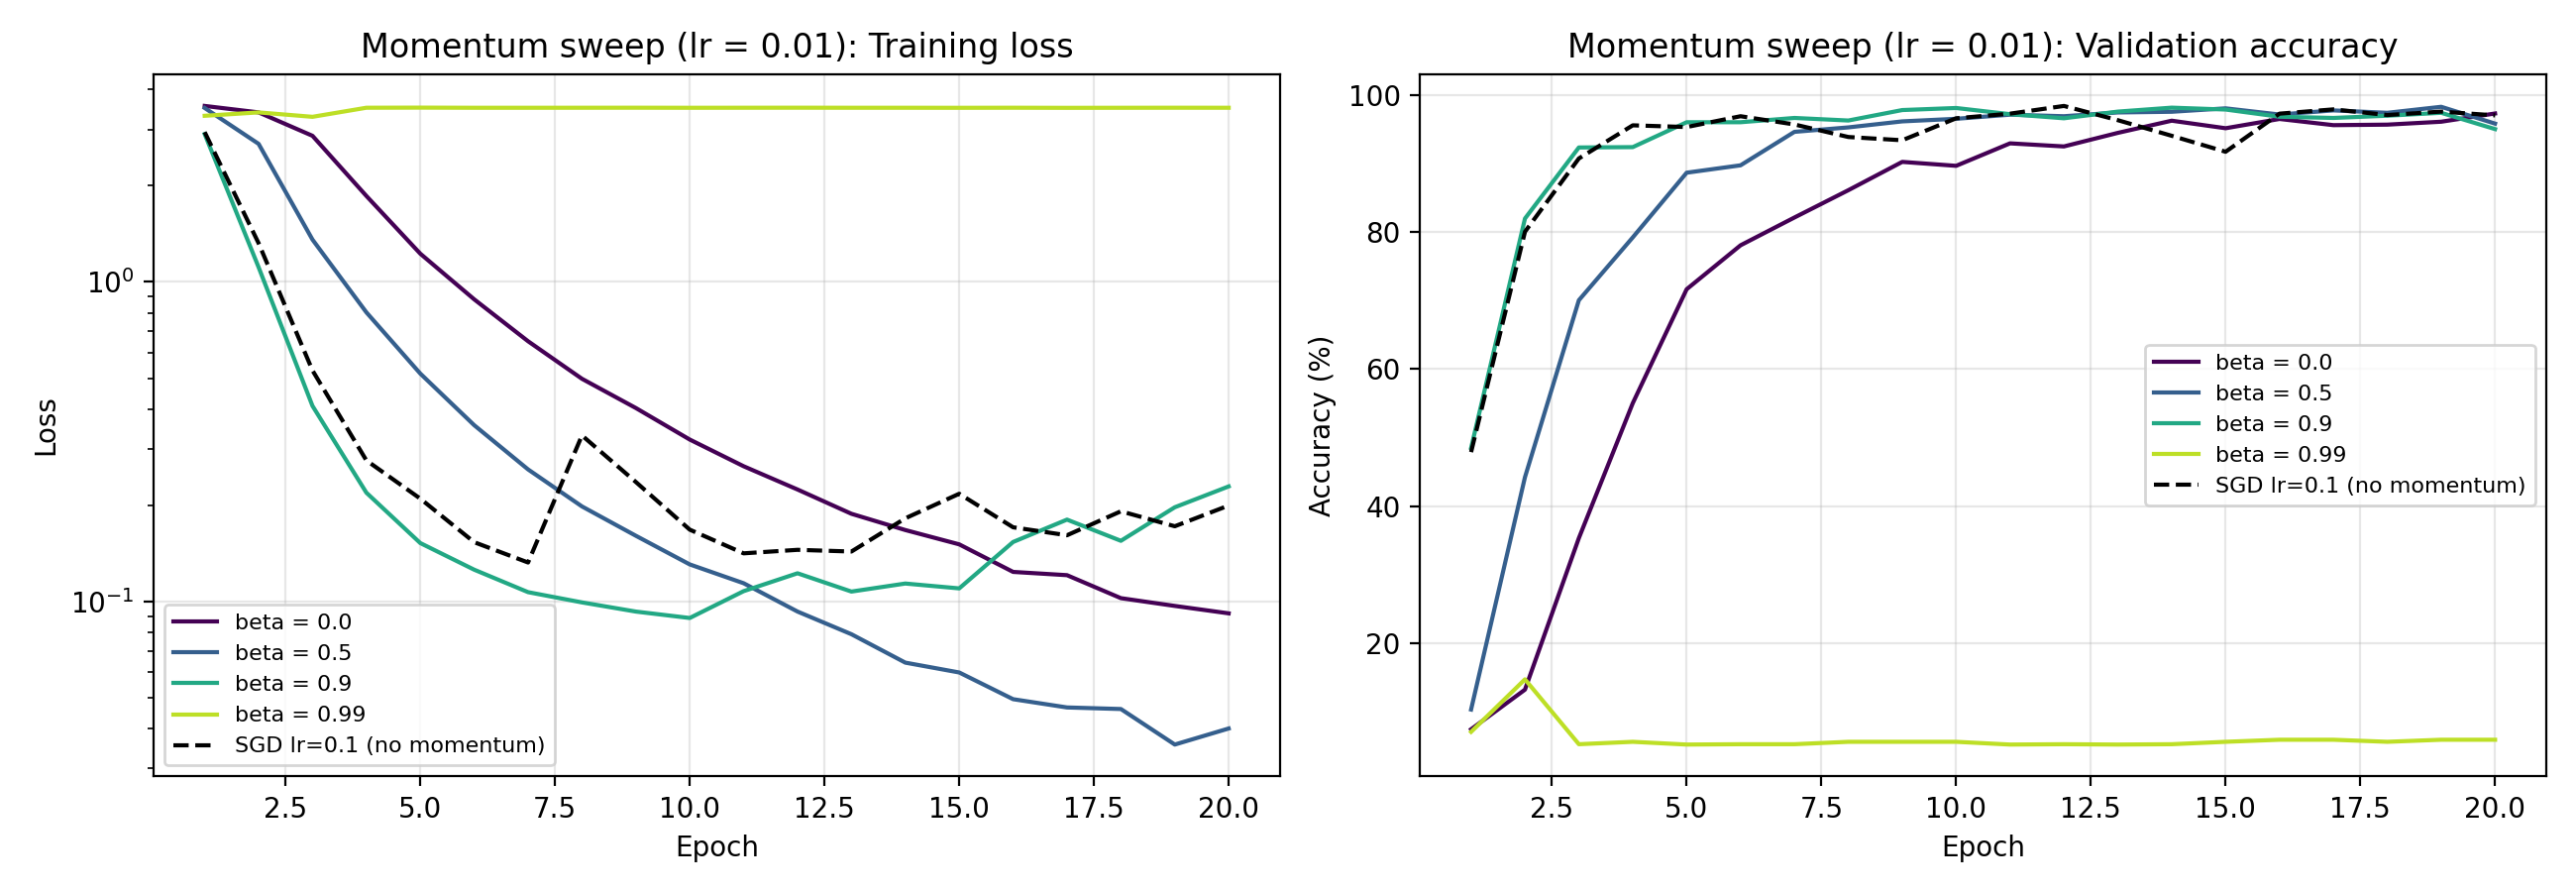
\includegraphics[width=\textwidth]{figures/momentum_sweep.png}
\caption{Momentum sweep at $\eta = 0.01$: training loss (log scale) and validation accuracy. The dashed line is the
plain-SGD control run with $\eta = 0.1$, the same effective step size as $\beta = 0.9$.}
\label{fig:momentum}
\end{figure}

% ==========================================
\section{Custom Model Training and Evaluation}
% ==========================================

\subsection{Training Set-up}

Both custom models were trained with an identical pipeline (Table~\ref{tab:setup}), so the comparison isolates the
effect of the convolution type.

\begin{table}[H]
\centering
\caption{Training set-up for Models A and B.}
\label{tab:setup}
\begin{tabular}{ll}
\toprule
Loss              & Cross-entropy \\
Optimizer         & Adam, $\eta = 0.001$ \\
Epochs / batch    & 25 / 32 \\
Weights tested    & Epoch with the lowest validation loss \\
Reproducibility   & Seed 42, deterministic cuDNN \\
Hardware          & NVIDIA GTX 1660 Ti \\
Epoch timing      & Median over all epochs, after an untimed pass that reads every image once \\
\bottomrule
\end{tabular}
\end{table}

The median epoch time is reported because an earlier run showed that a single epoch can be slowed 2--3$\times$ by the
first read of the dataset from disk or by other activity on the computer; the median is not affected by such outliers.

\subsection{Training and Validation Loss}

\begin{figure}[H]
\centering
\begin{subfigure}{0.49\textwidth}
    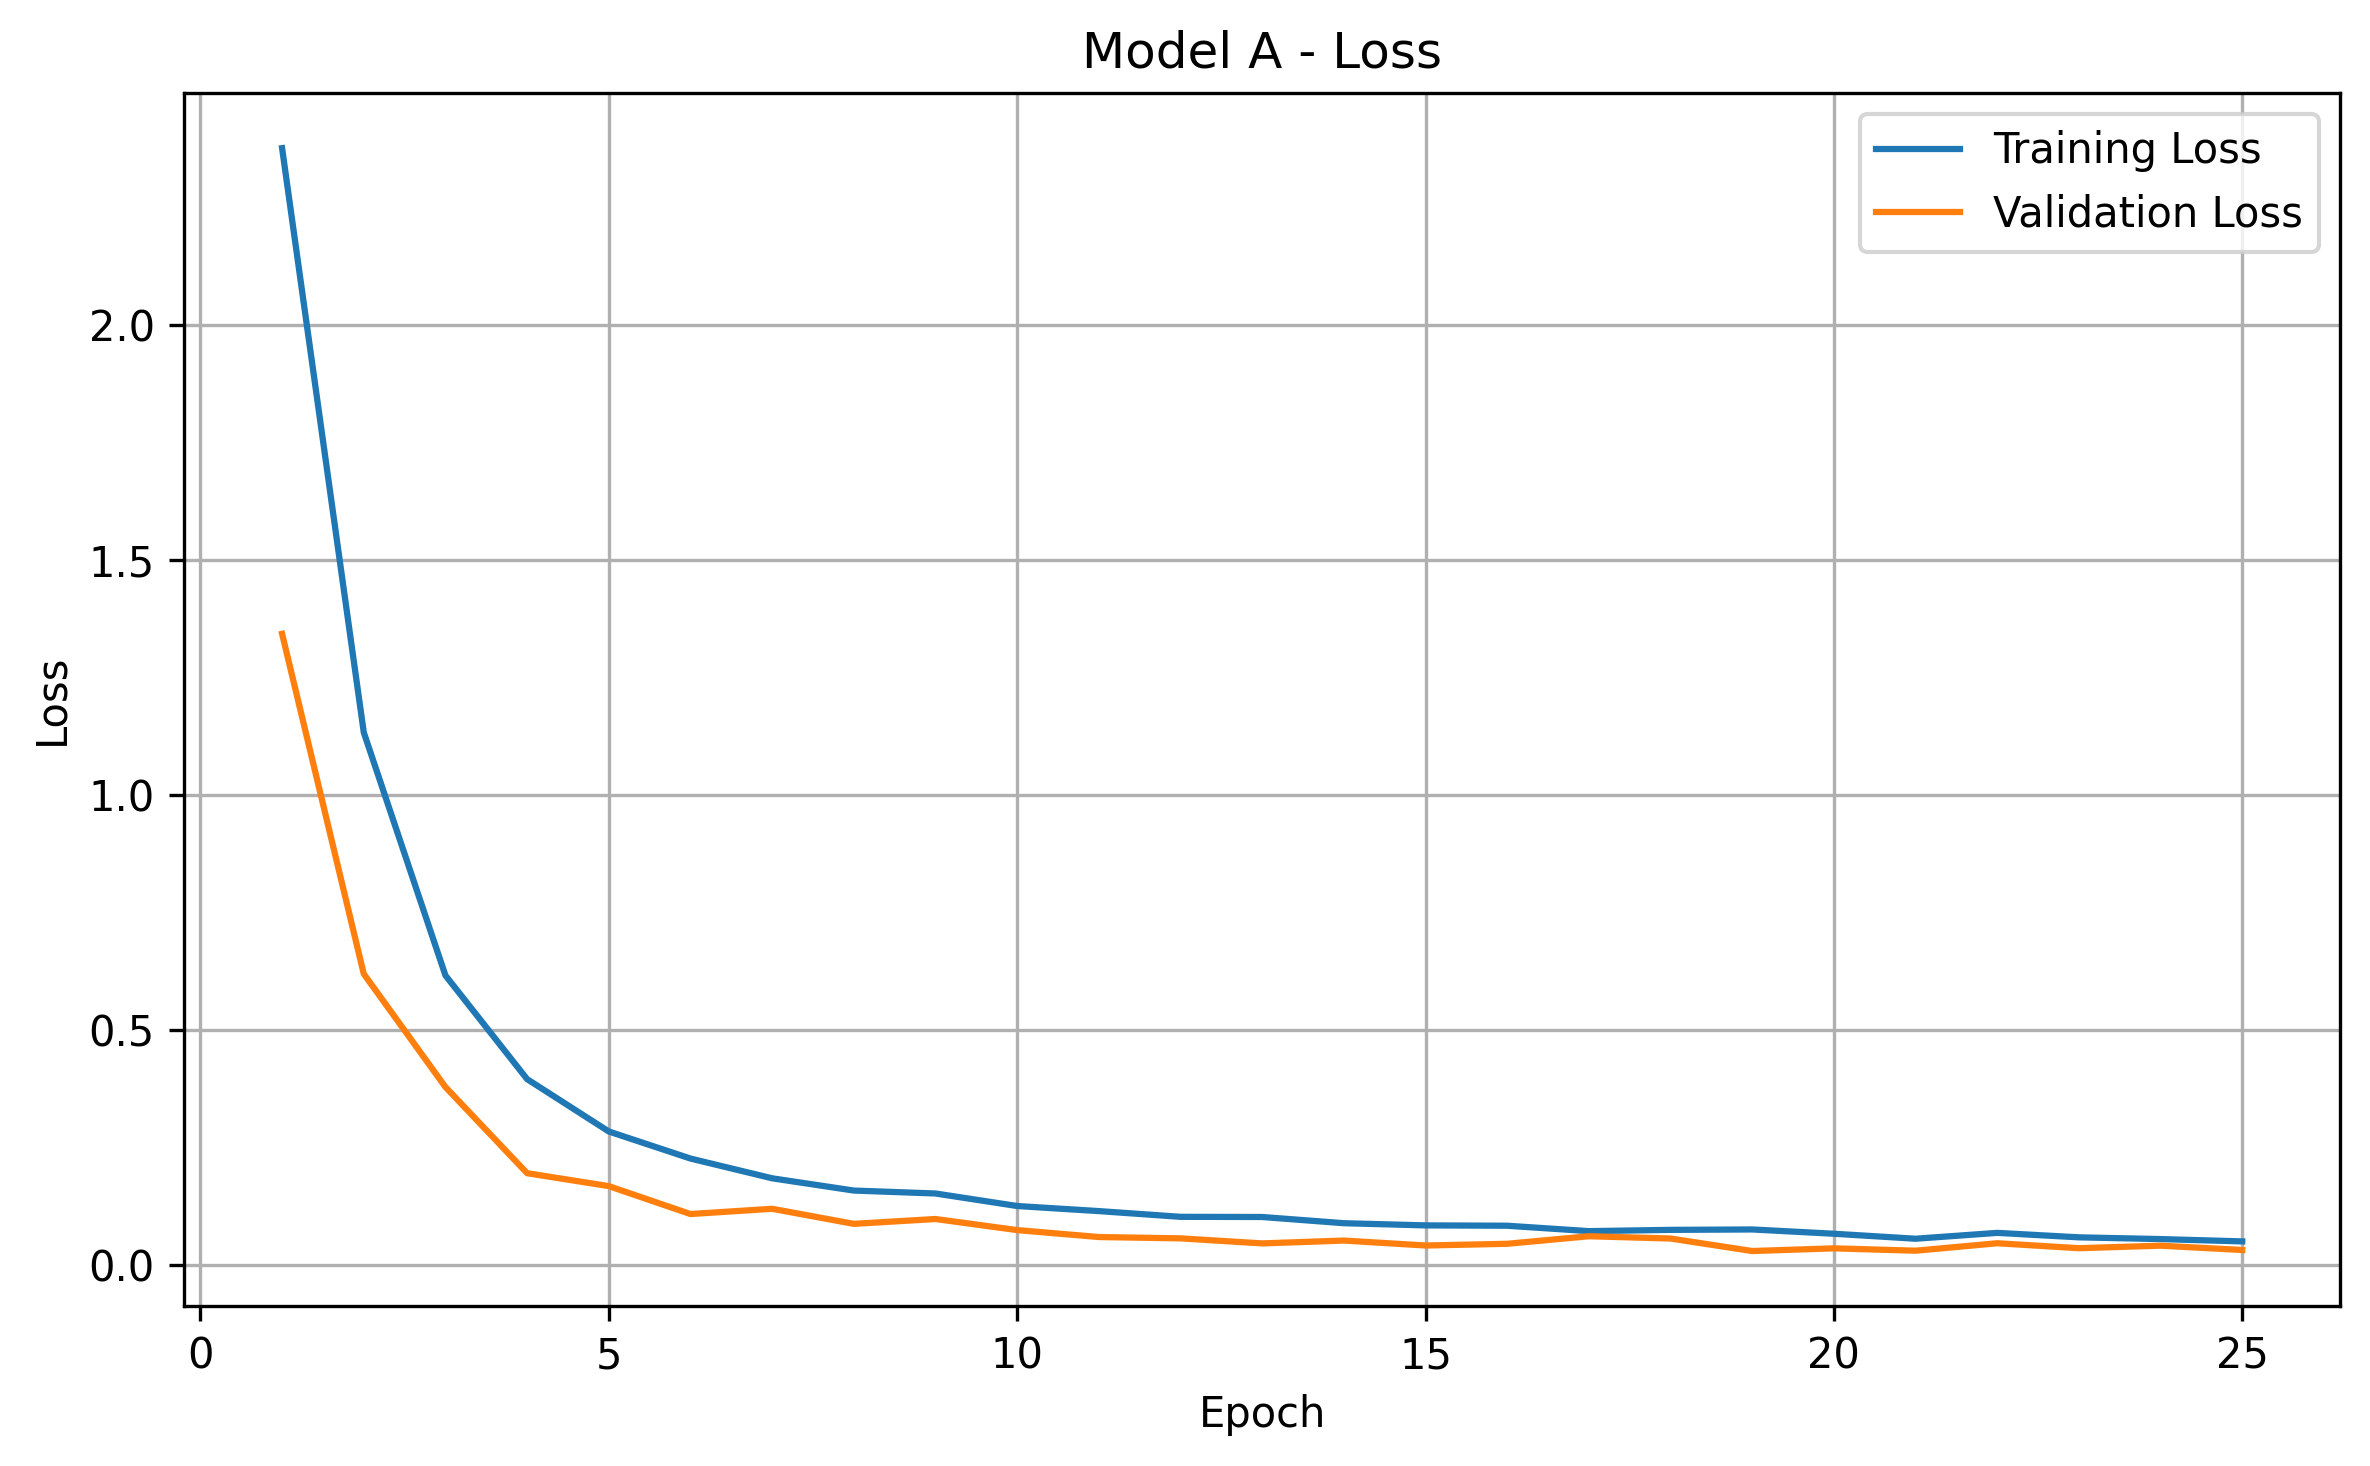
\includegraphics[width=\textwidth]{figures/model_a_loss.png}
    \caption{Model A}
\end{subfigure}
\hfill
\begin{subfigure}{0.49\textwidth}
    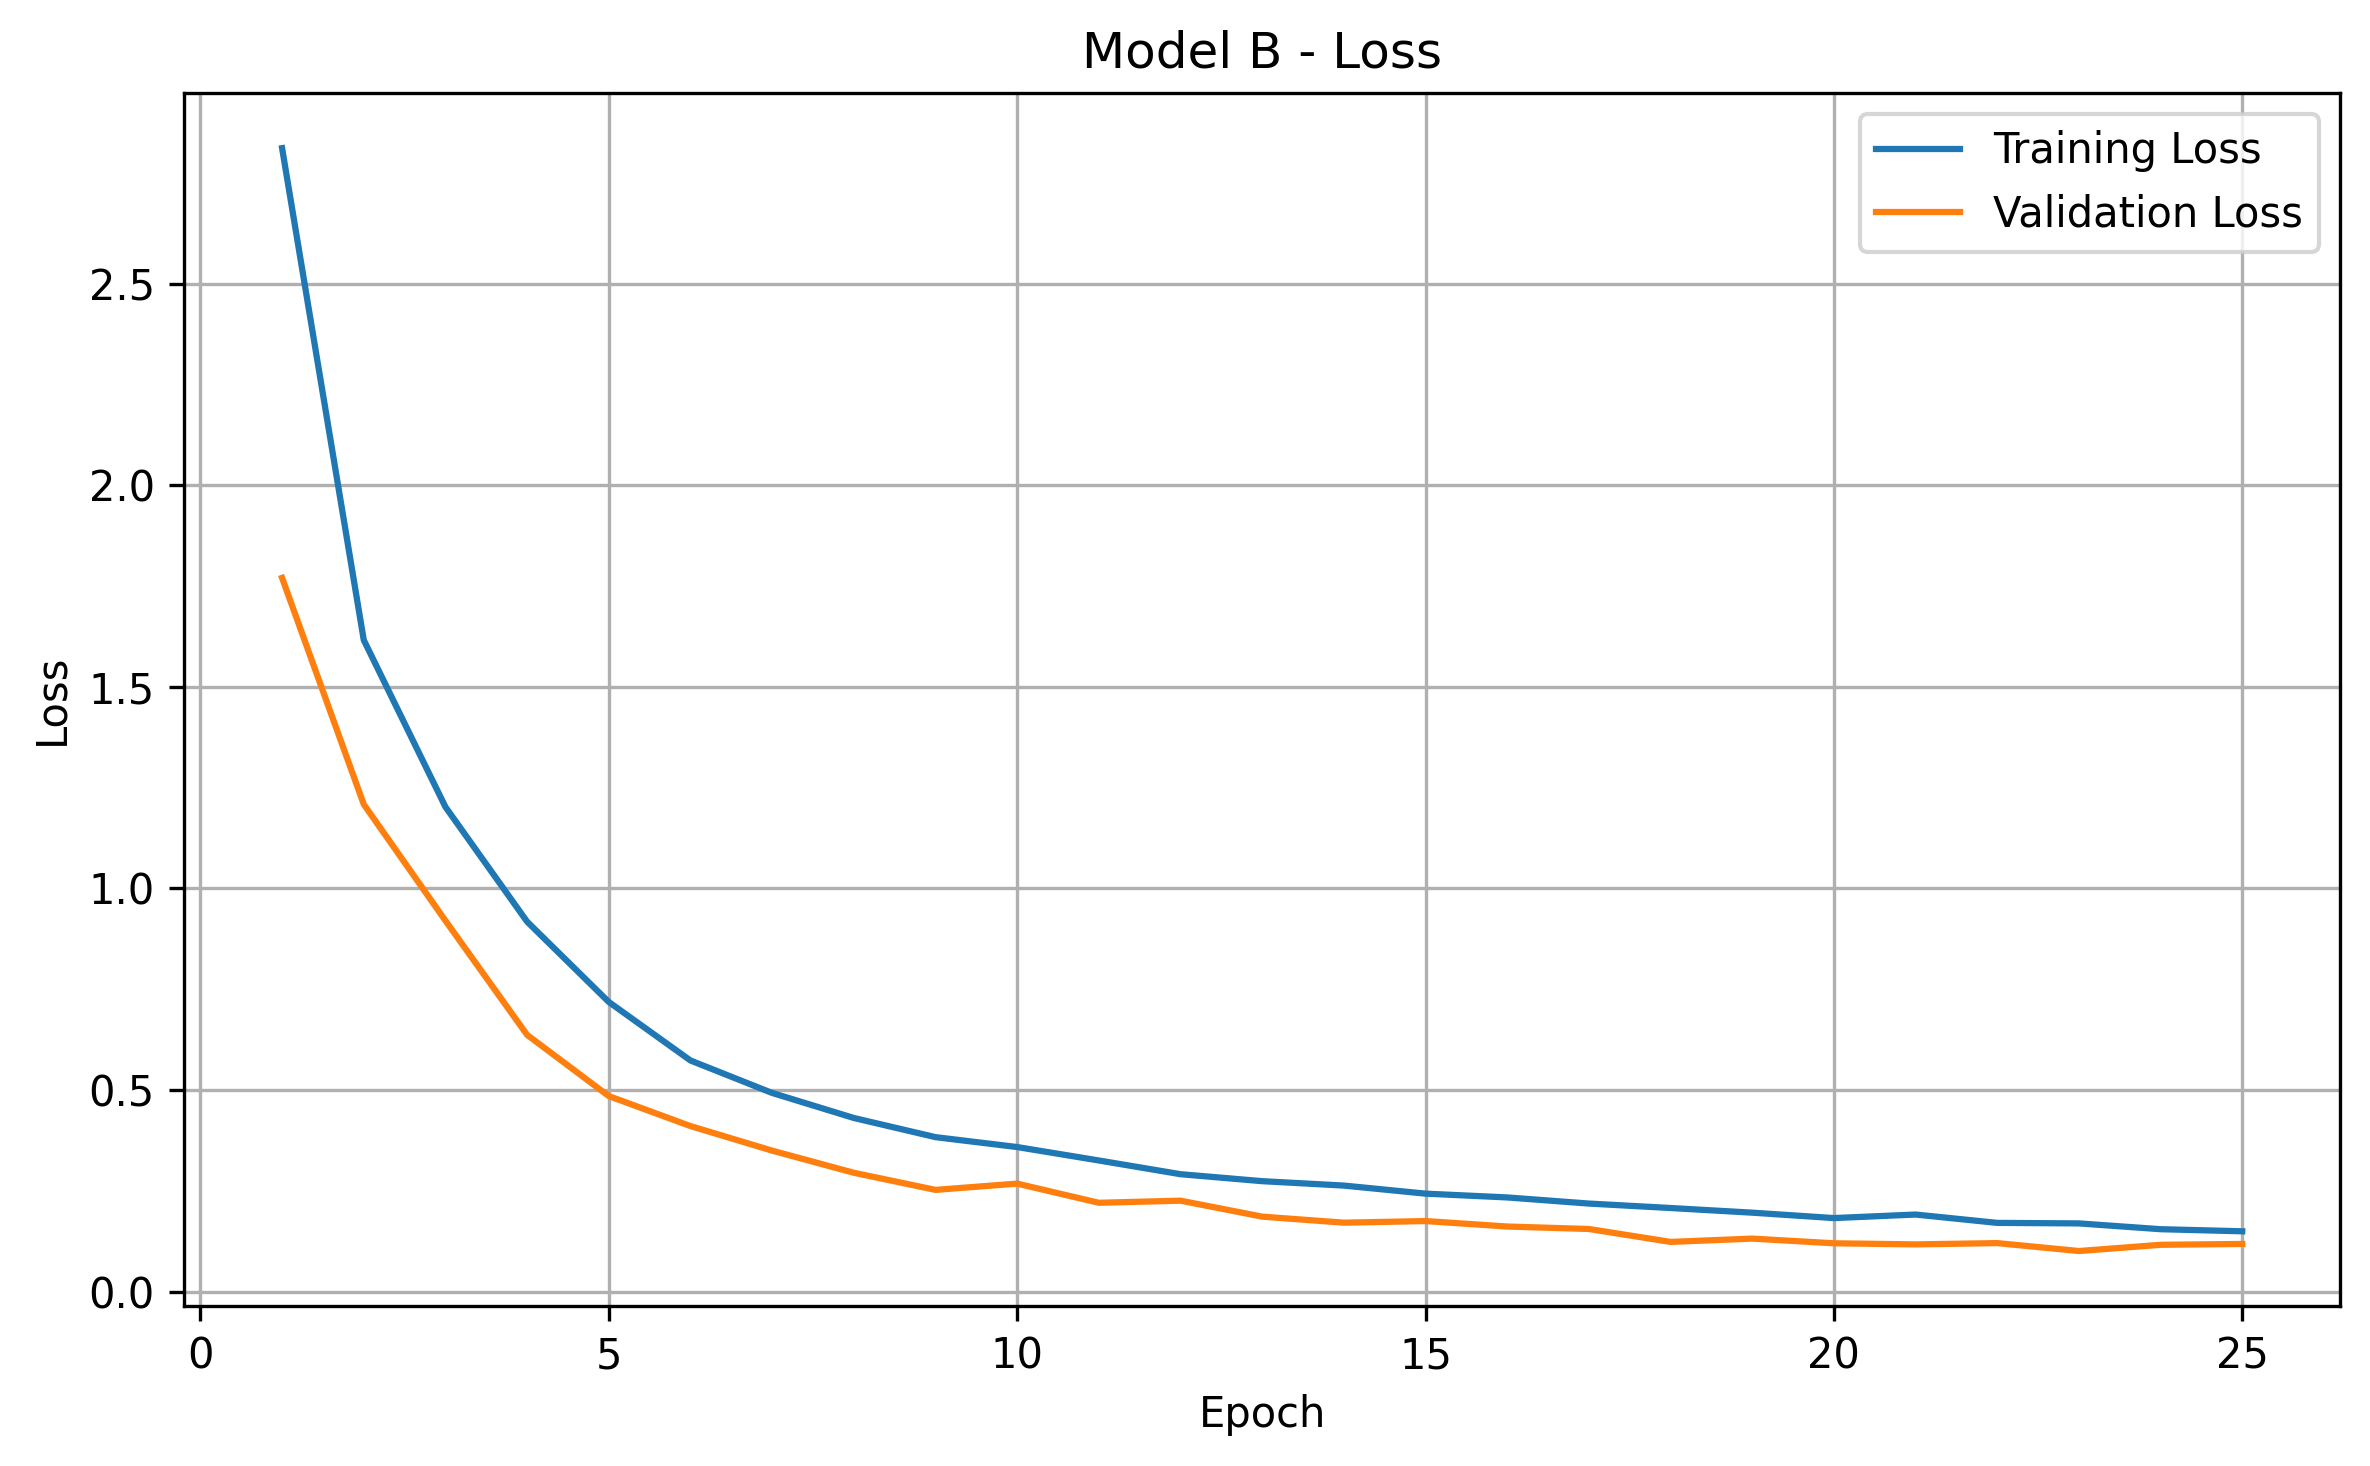
\includegraphics[width=\textwidth]{figures/model_b_loss.png}
    \caption{Model B}
\end{subfigure}
\caption{Training and validation loss over 25 epochs.}
\label{fig:loss}
\end{figure}

Both models converge smoothly and show \textbf{no overfitting} (Figure~\ref{fig:loss}): the validation loss keeps
decreasing and stays below the training loss in every epoch. The training loss is higher because it is measured on augmented images, which are harder than the
unaltered validation images. Model A reaches 95\% validation accuracy at epoch 6 and its best validation loss
(0.029) at epoch 19. Model B learns more slowly (95\% only at epoch 16), is still improving at epoch 25 (best
validation loss 0.100 at epoch 23) and never reaches 99\% validation accuracy, which indicates that it is limited by
its capacity rather than by overfitting (Figure~\ref{fig:abcurves}).

\begin{figure}[H]
\centering
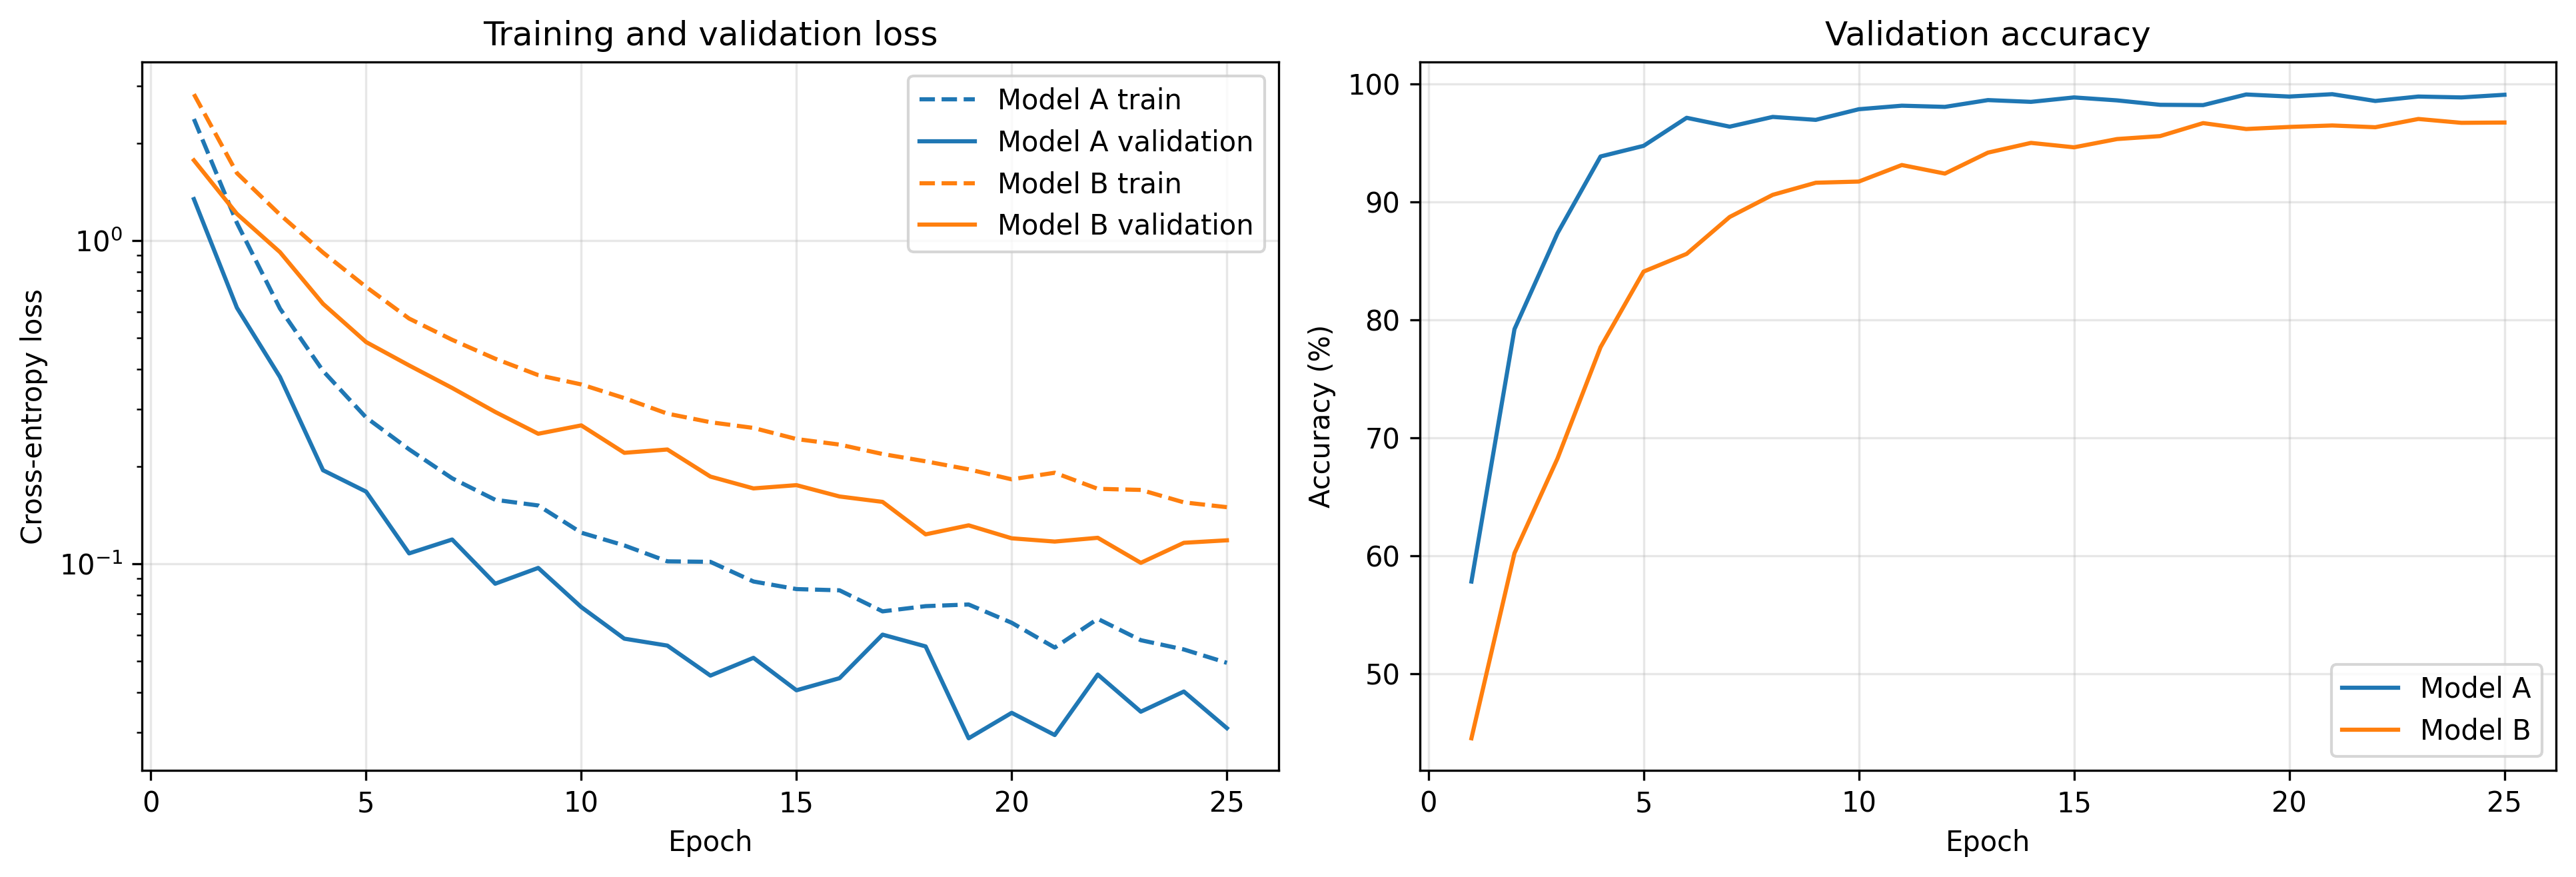
\includegraphics[width=\textwidth]{figures/model_a_vs_model_b_loss.png}
\caption{Model A vs Model B: training (dashed) and validation (solid) loss, and validation accuracy.}
\label{fig:abcurves}
\end{figure}

\subsection{Test-Set Evaluation}

\begin{table}[H]
\centering
\caption{Test-set results (3,996 images). Precision and recall are macro-averaged over the 43 classes.}
\label{tab:testab}
\begin{tabular}{lrrrr}
\toprule
\textbf{Model} & \textbf{Accuracy (\%)} & \textbf{Precision (\%)} & \textbf{Recall (\%)} & \textbf{Misclassified} \\
\midrule
Model A & 98.97 & 98.74 & 99.17 & 41 \\
Model B & 97.00 & 97.49 & 97.36 & 120 \\
\bottomrule
\end{tabular}
\end{table}

\begin{figure}[H]
\centering
\begin{subfigure}{0.49\textwidth}
    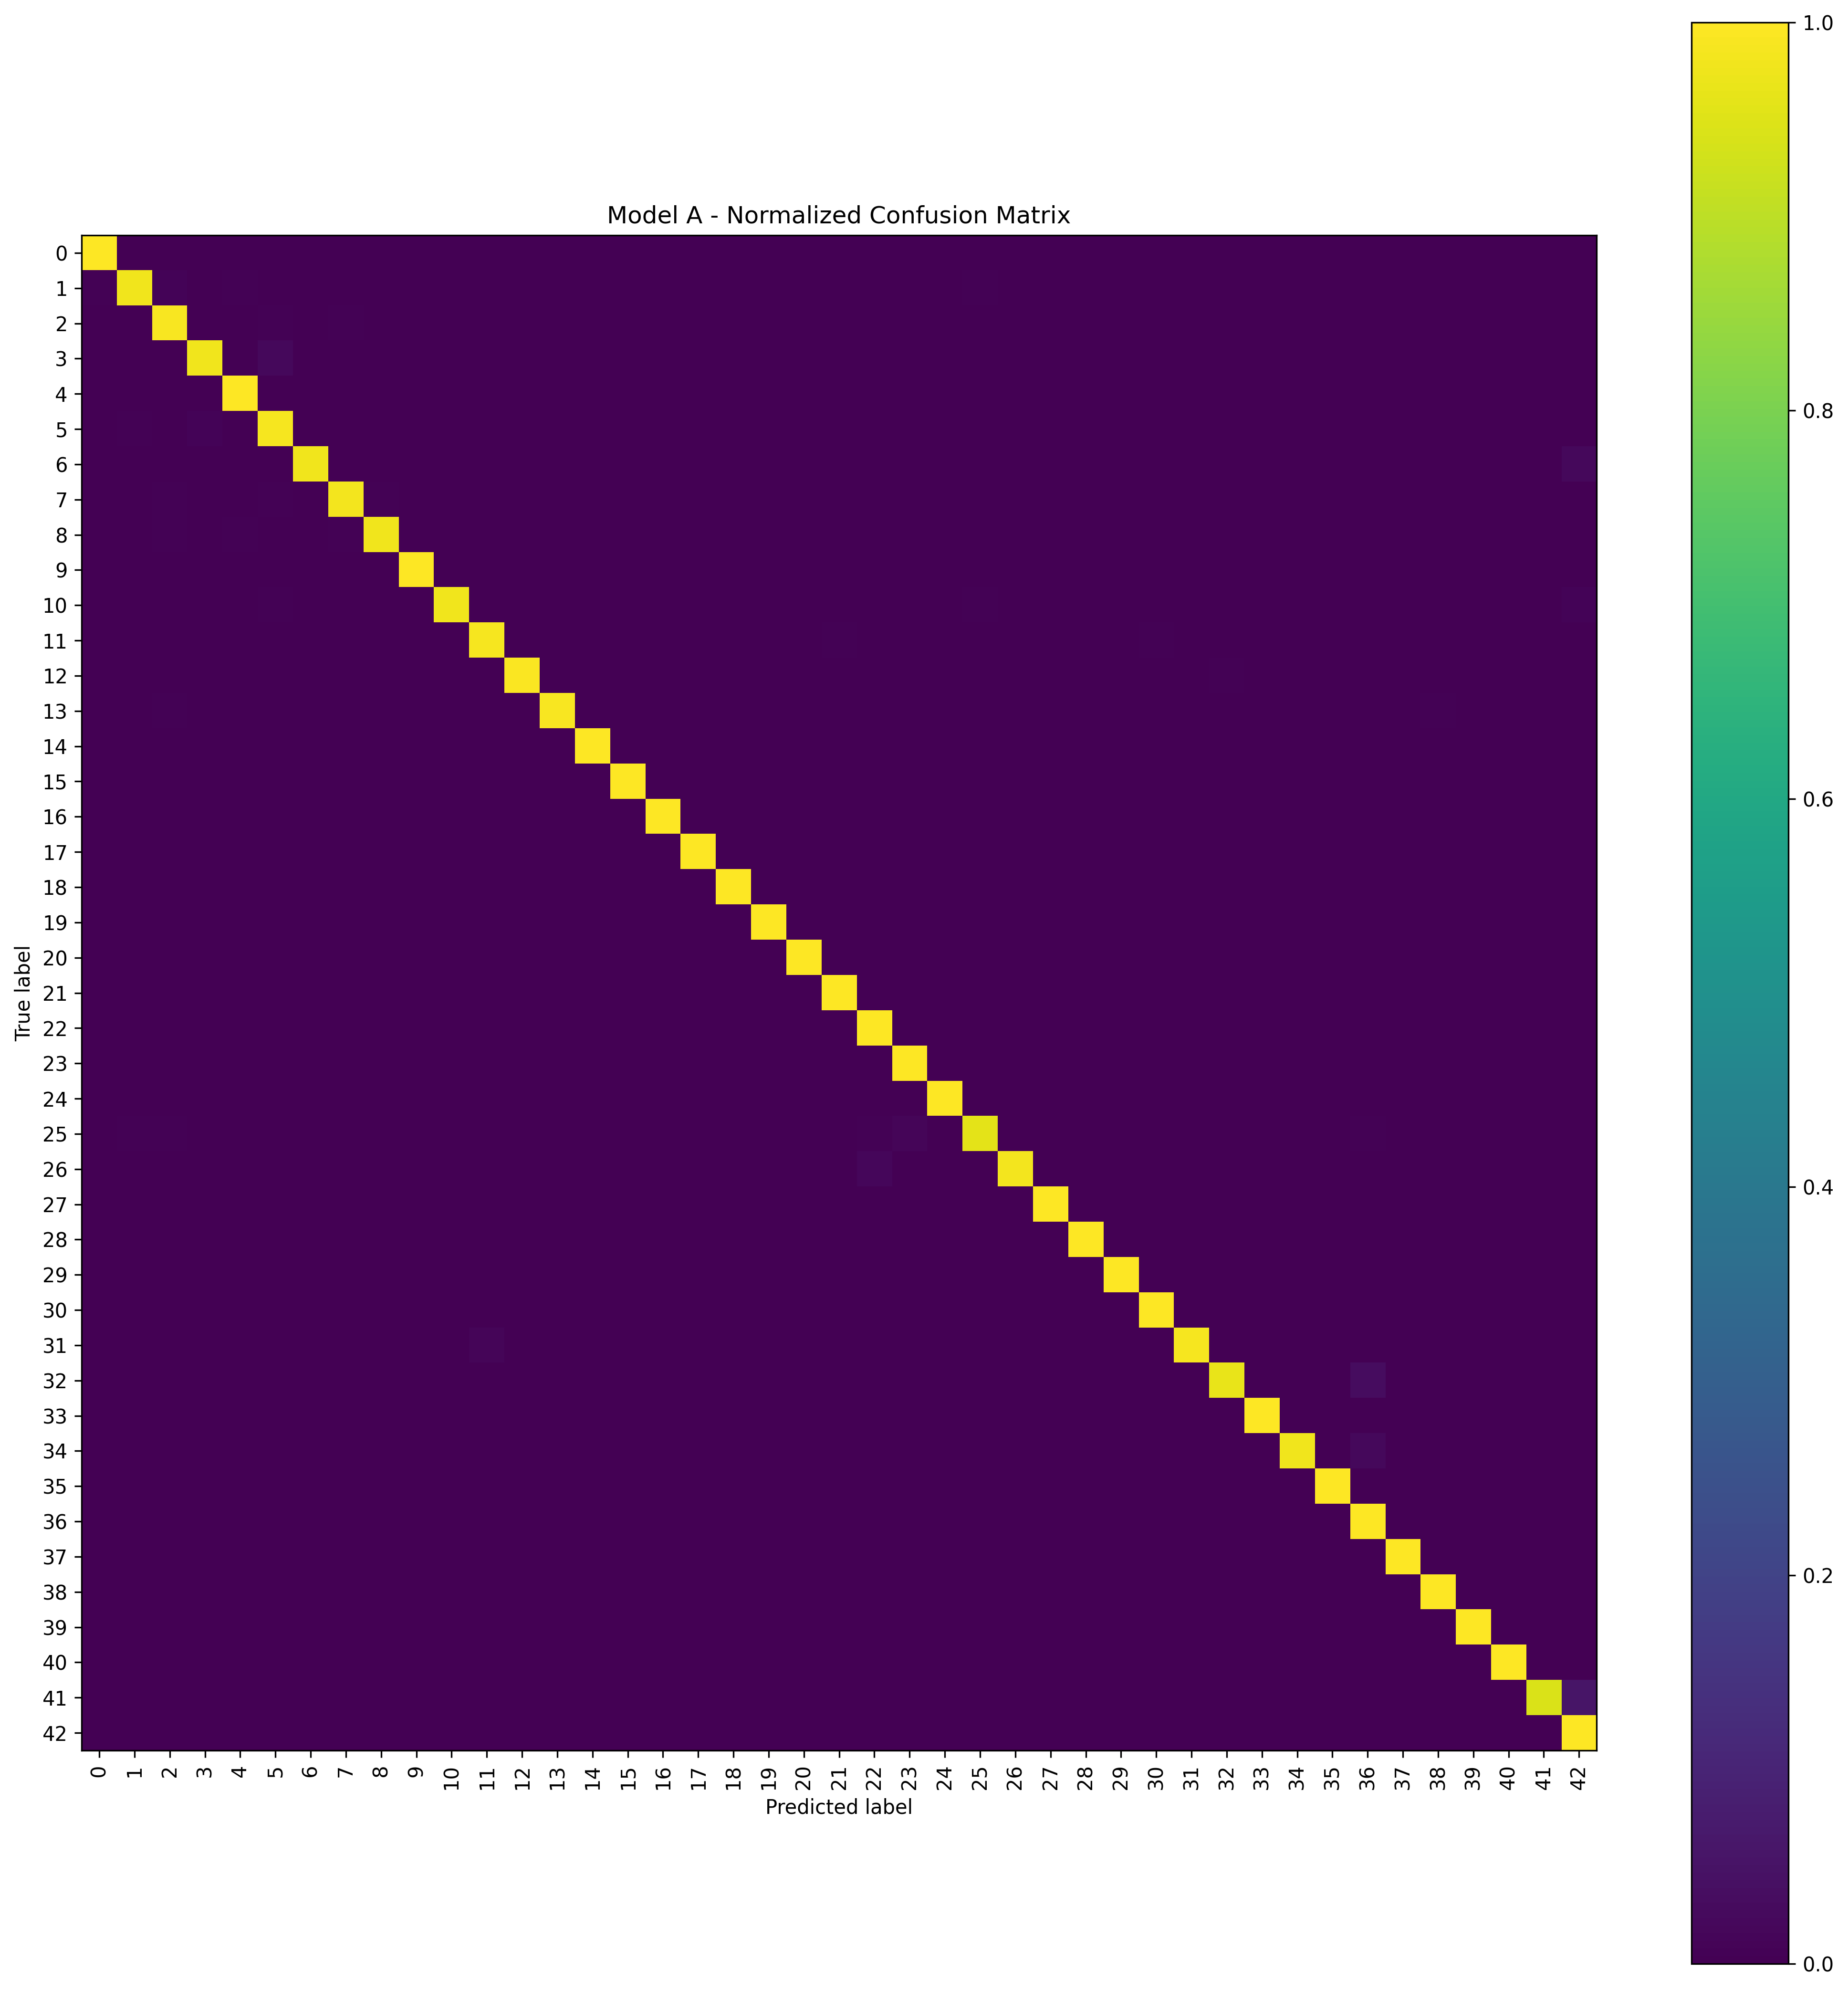
\includegraphics[width=\textwidth]{figures/model_a_confusion_matrix.png}
    \caption{Model A}
\end{subfigure}
\hfill
\begin{subfigure}{0.49\textwidth}
    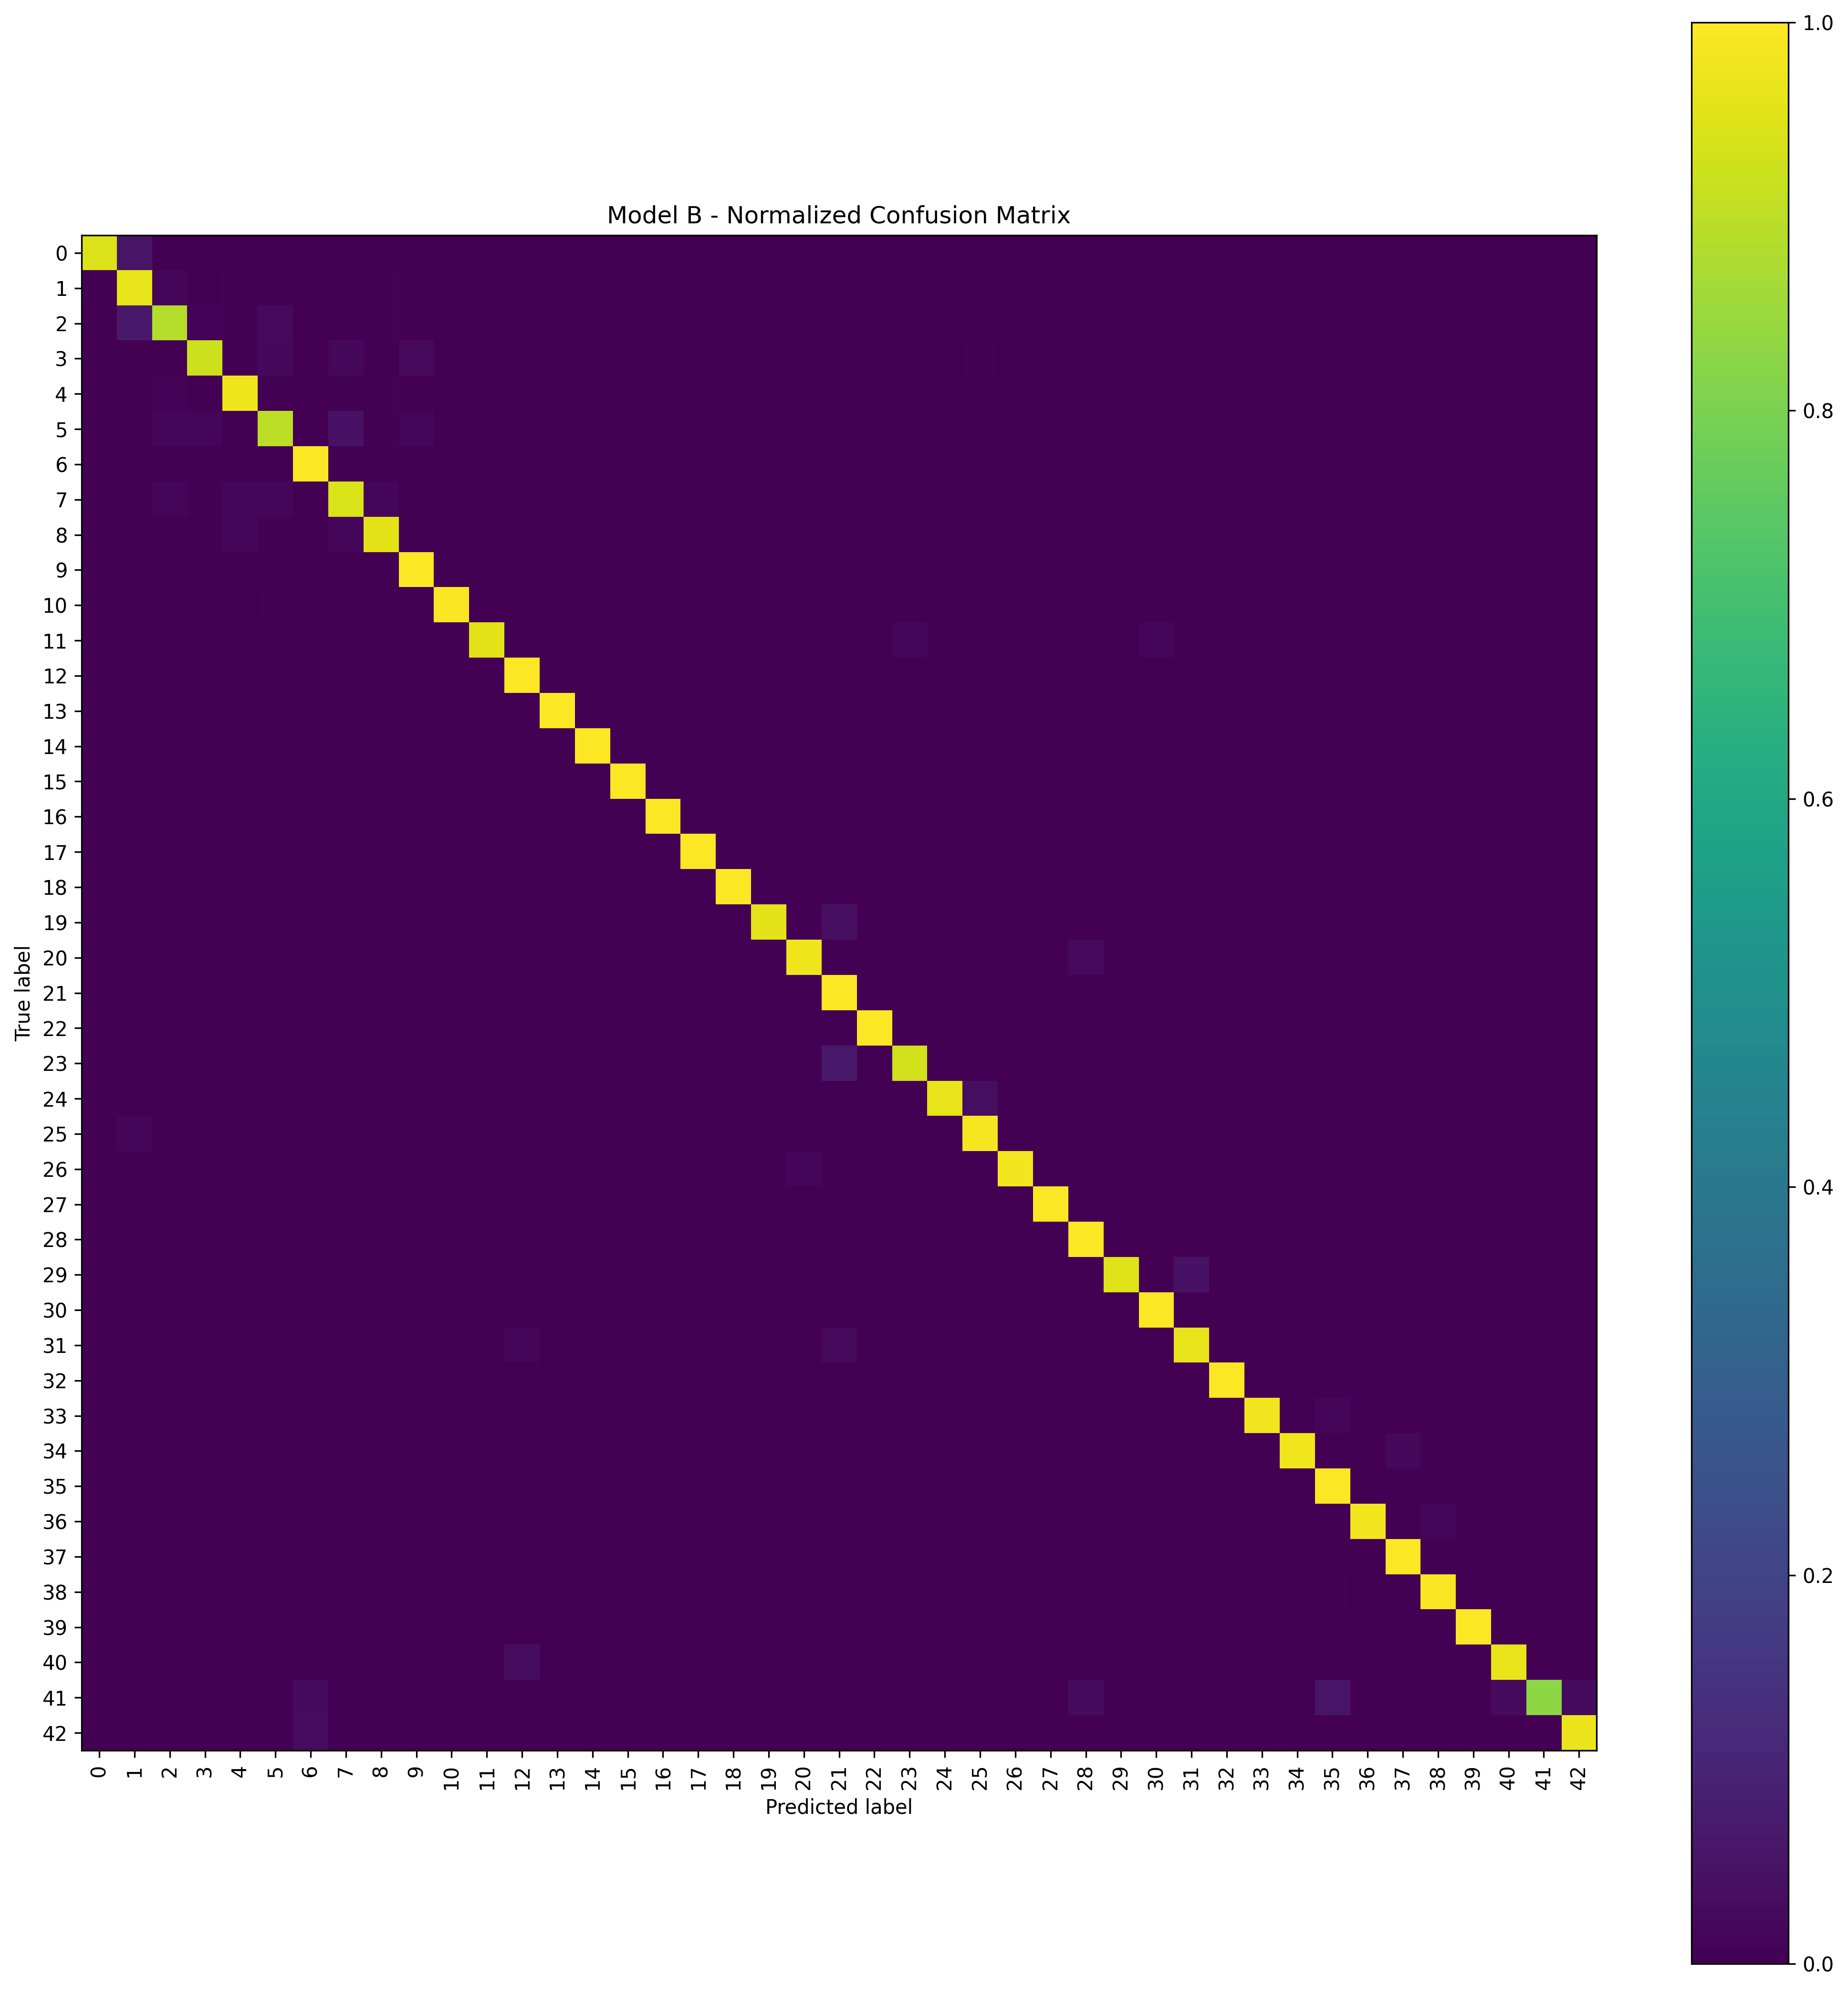
\includegraphics[width=\textwidth]{figures/model_b_confusion_matrix.png}
    \caption{Model B}
\end{subfigure}
\caption{Row-normalised confusion matrices on the test set (true class vs predicted class).}
\label{fig:cm}
\end{figure}

Model A misclassifies 41 of the 3,996 test images and Model B 120 (Table~\ref{tab:testab}). Both confusion matrices
(Figure~\ref{fig:cm}) are strongly diagonal. The remaining errors concentrate in the top-left block of
\textbf{speed-limit signs} (classes 0--8), which share the same red circle and differ only in their digits. Model B's
most frequent error is predicting \emph{30\,km/h} for a \emph{50\,km/h} sign (16 times), and its lowest recalls are
for 50\,km/h (88.8\%), 80\,km/h (90.0\%) and 60\,km/h (92.6\%), together with \emph{end of no passing}
(class 41, 82.9\%, a rare class with 35 test images). Signs with distinctive shapes or colours, such as stop, yield
or no entry, are classified almost perfectly by both models.

\subsection{Model A vs Model B}

\begin{table}[H]
\centering
\caption{Comparison of the two custom models.}
\label{tab:ab}
\begin{tabular}{lrrr}
\toprule
\textbf{Metric} & \textbf{Model A} & \textbf{Model B} & \textbf{Change} \\
\midrule
Trainable parameters             & 45,643     & 25,526     & $-44.1\%$ \\
Model size on disk (KB)          & 182.8      & 105.7      & $-42.2\%$ \\
MACs per image                   & 9.46\,M    & 1.42\,M    & $-85.0\%$ \\
Training time per epoch (s)      & 41.0       & 44.2       & $+7.8\%$ \\
GPU inference (ms/image)         & 0.36       & 0.34       & $-4.9\%$ \\
Test accuracy (\%)               & 98.97      & 97.00      & $-1.98$ pts \\
\bottomrule
\end{tabular}
\end{table}

\textbf{Trade-offs when moving to depthwise separable convolutions} (Table~\ref{tab:ab}):
\begin{itemize}
    \item \textbf{Memory and computation drop sharply.} Model B is 42\% smaller on disk and needs 85\% fewer MACs. In
          8-bit form it would need only about 25\,KB, small enough for the flash memory of a microcontroller.
    \item \textbf{Accuracy drops slightly.} The test accuracy falls by 2 percentage points (3$\times$ more errors).
          Separating spatial filtering from channel mixing reduces the model's capacity to learn fine,
          multi-channel patterns such as the digits on speed-limit signs.
    \item \textbf{Fewer MACs did not mean faster training on the GPU.} Model B is 7.8\% \emph{slower} per epoch.
          It has twice as many layers (eight convolutions instead of four), and each layer has a fixed launch and
          memory-transfer overhead. Depthwise convolutions perform very little arithmetic per value loaded, so a GPU
          cannot use its parallelism efficiently, and most of each epoch is spent loading images, which is identical
          for both models. Model B's single-thread CPU latency was likewise no lower than Model A's (1.61 vs 1.52\,ms,
          Section~\ref{sec:final}). The MAC savings only translate into real speed on hardware where arithmetic is the
          bottleneck and depthwise convolutions are optimised, for example microcontroller libraries such as
          CMSIS-NN or TensorFlow Lite Micro.
    \item \textbf{Slower convergence.} Model B needs about three times as many epochs to reach 95\% validation accuracy.
\end{itemize}

% ==========================================
\section{Fine-Tuning Lightweight State-of-the-Art Networks}
% ==========================================

\subsection{Selected Models}

\begin{itemize}
    \item \textbf{MobileNetV2} \cite{mobilenetv2} is built from inverted residual blocks: a $1 \times 1$ expansion,
          a depthwise $3 \times 3$ convolution and a linear $1 \times 1$ projection, with ReLU6 activations
          ($\min(\max(0, x), 6)$), which are cheap and bounded, and therefore quantisation friendly.
    \item \textbf{EfficientNet-B0} \cite{efficientnet} uses MBConv blocks (the same inverted-residual idea) with
          squeeze-and-excitation attention, and its depth, width and resolution were found by neural architecture
          search. It uses SiLU (Swish) activations, $x \cdot \sigma(x)$, and sigmoid gates, which need an exponential for
          every value.
\end{itemize}

\subsection{Fine-Tuning Procedure}

Both networks were loaded with ImageNet weights, their 1000-class output layer was replaced by a new
$1280 \rightarrow 43$ linear layer, and they were trained with an identical recipe on the same splits and
augmentation as the custom models:
\begin{enumerate}
    \item \textbf{Head warm-up (3 epochs):} the pretrained backbone is frozen and only the new head is trained (Adam,
          $\eta = 10^{-3}$), so its random initial gradients cannot damage the pretrained features.
    \item \textbf{Full fine-tuning (17 epochs):} all layers are unfrozen and trained with Adam at a 10$\times$ smaller
          learning rate ($\eta = 10^{-4}$) with cosine decay.
\end{enumerate}
The input was kept at $64 \times 64$ rather than upsampled to the networks' native $224 \times 224$: upsampling adds
no information but would multiply the computation by about $(224/64)^2 \approx 12$, which defeats the purpose of an
edge model. The weights with the lowest validation loss were used for testing.

\begin{table}[H]
\centering
\caption{Fine-tuned SOTA models (test set: 3,996 images).}
\label{tab:sota}
\begin{tabular}{lrr}
\toprule
\textbf{Metric} & \textbf{MobileNetV2} & \textbf{EfficientNet-B0} \\
\midrule
Total parameters (all trainable)   & 2,278,955 & 4,062,631 \\
\quad of which new 43-class head    & 55,083    & 55,083 \\
Model size on disk (MB)             & 8.93      & 15.79 \\
MACs per $64 \times 64$ image       & 24.50\,M  & 32.02\,M \\
Test accuracy (\%)                  & 100.00    & 99.82 \\
Macro precision / recall (\%)       & 100.00 / 100.00 & 99.87 / 99.91 \\
Misclassified test images           & 0         & 7 \\
First epoch with $\geq 99\%$ val.\ accuracy & 7 & 8 \\
Training time per epoch, full fine-tuning (s) & 55.8 & 70.1 \\
\bottomrule
\end{tabular}
\end{table}

\begin{figure}[H]
\centering
\begin{subfigure}{0.49\textwidth}
    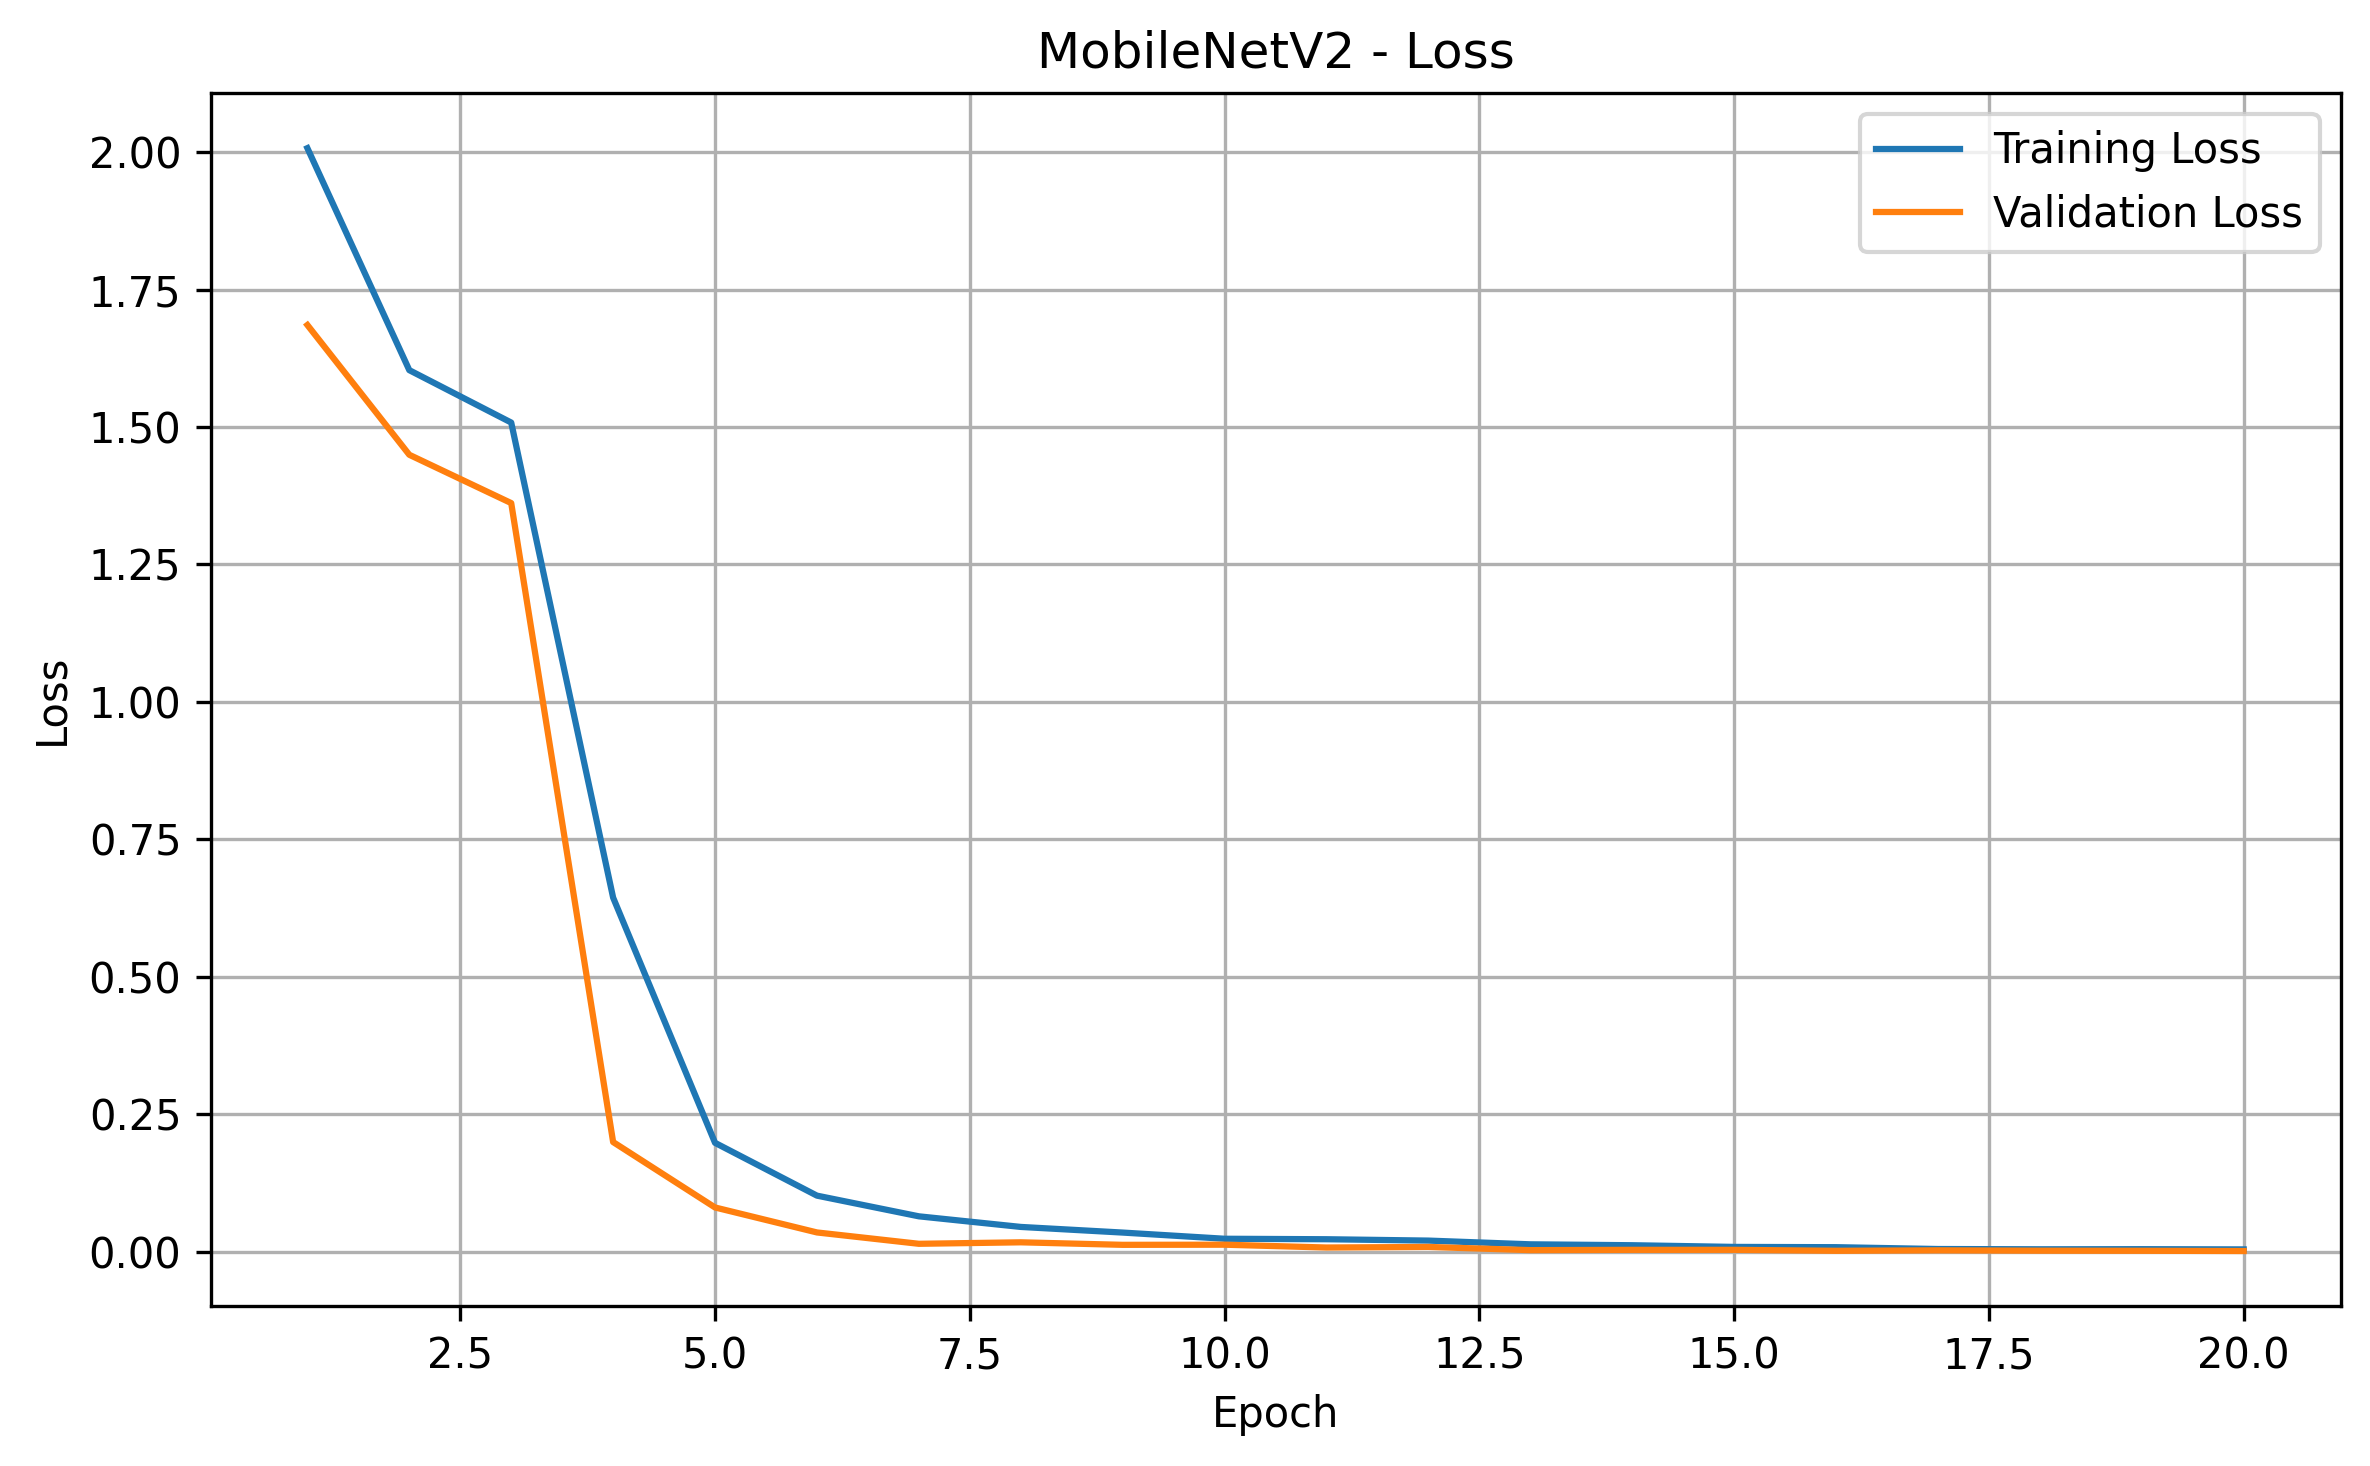
\includegraphics[width=\textwidth]{figures/mobilenetv2_loss.png}
    \caption{MobileNetV2}
\end{subfigure}
\hfill
\begin{subfigure}{0.49\textwidth}
    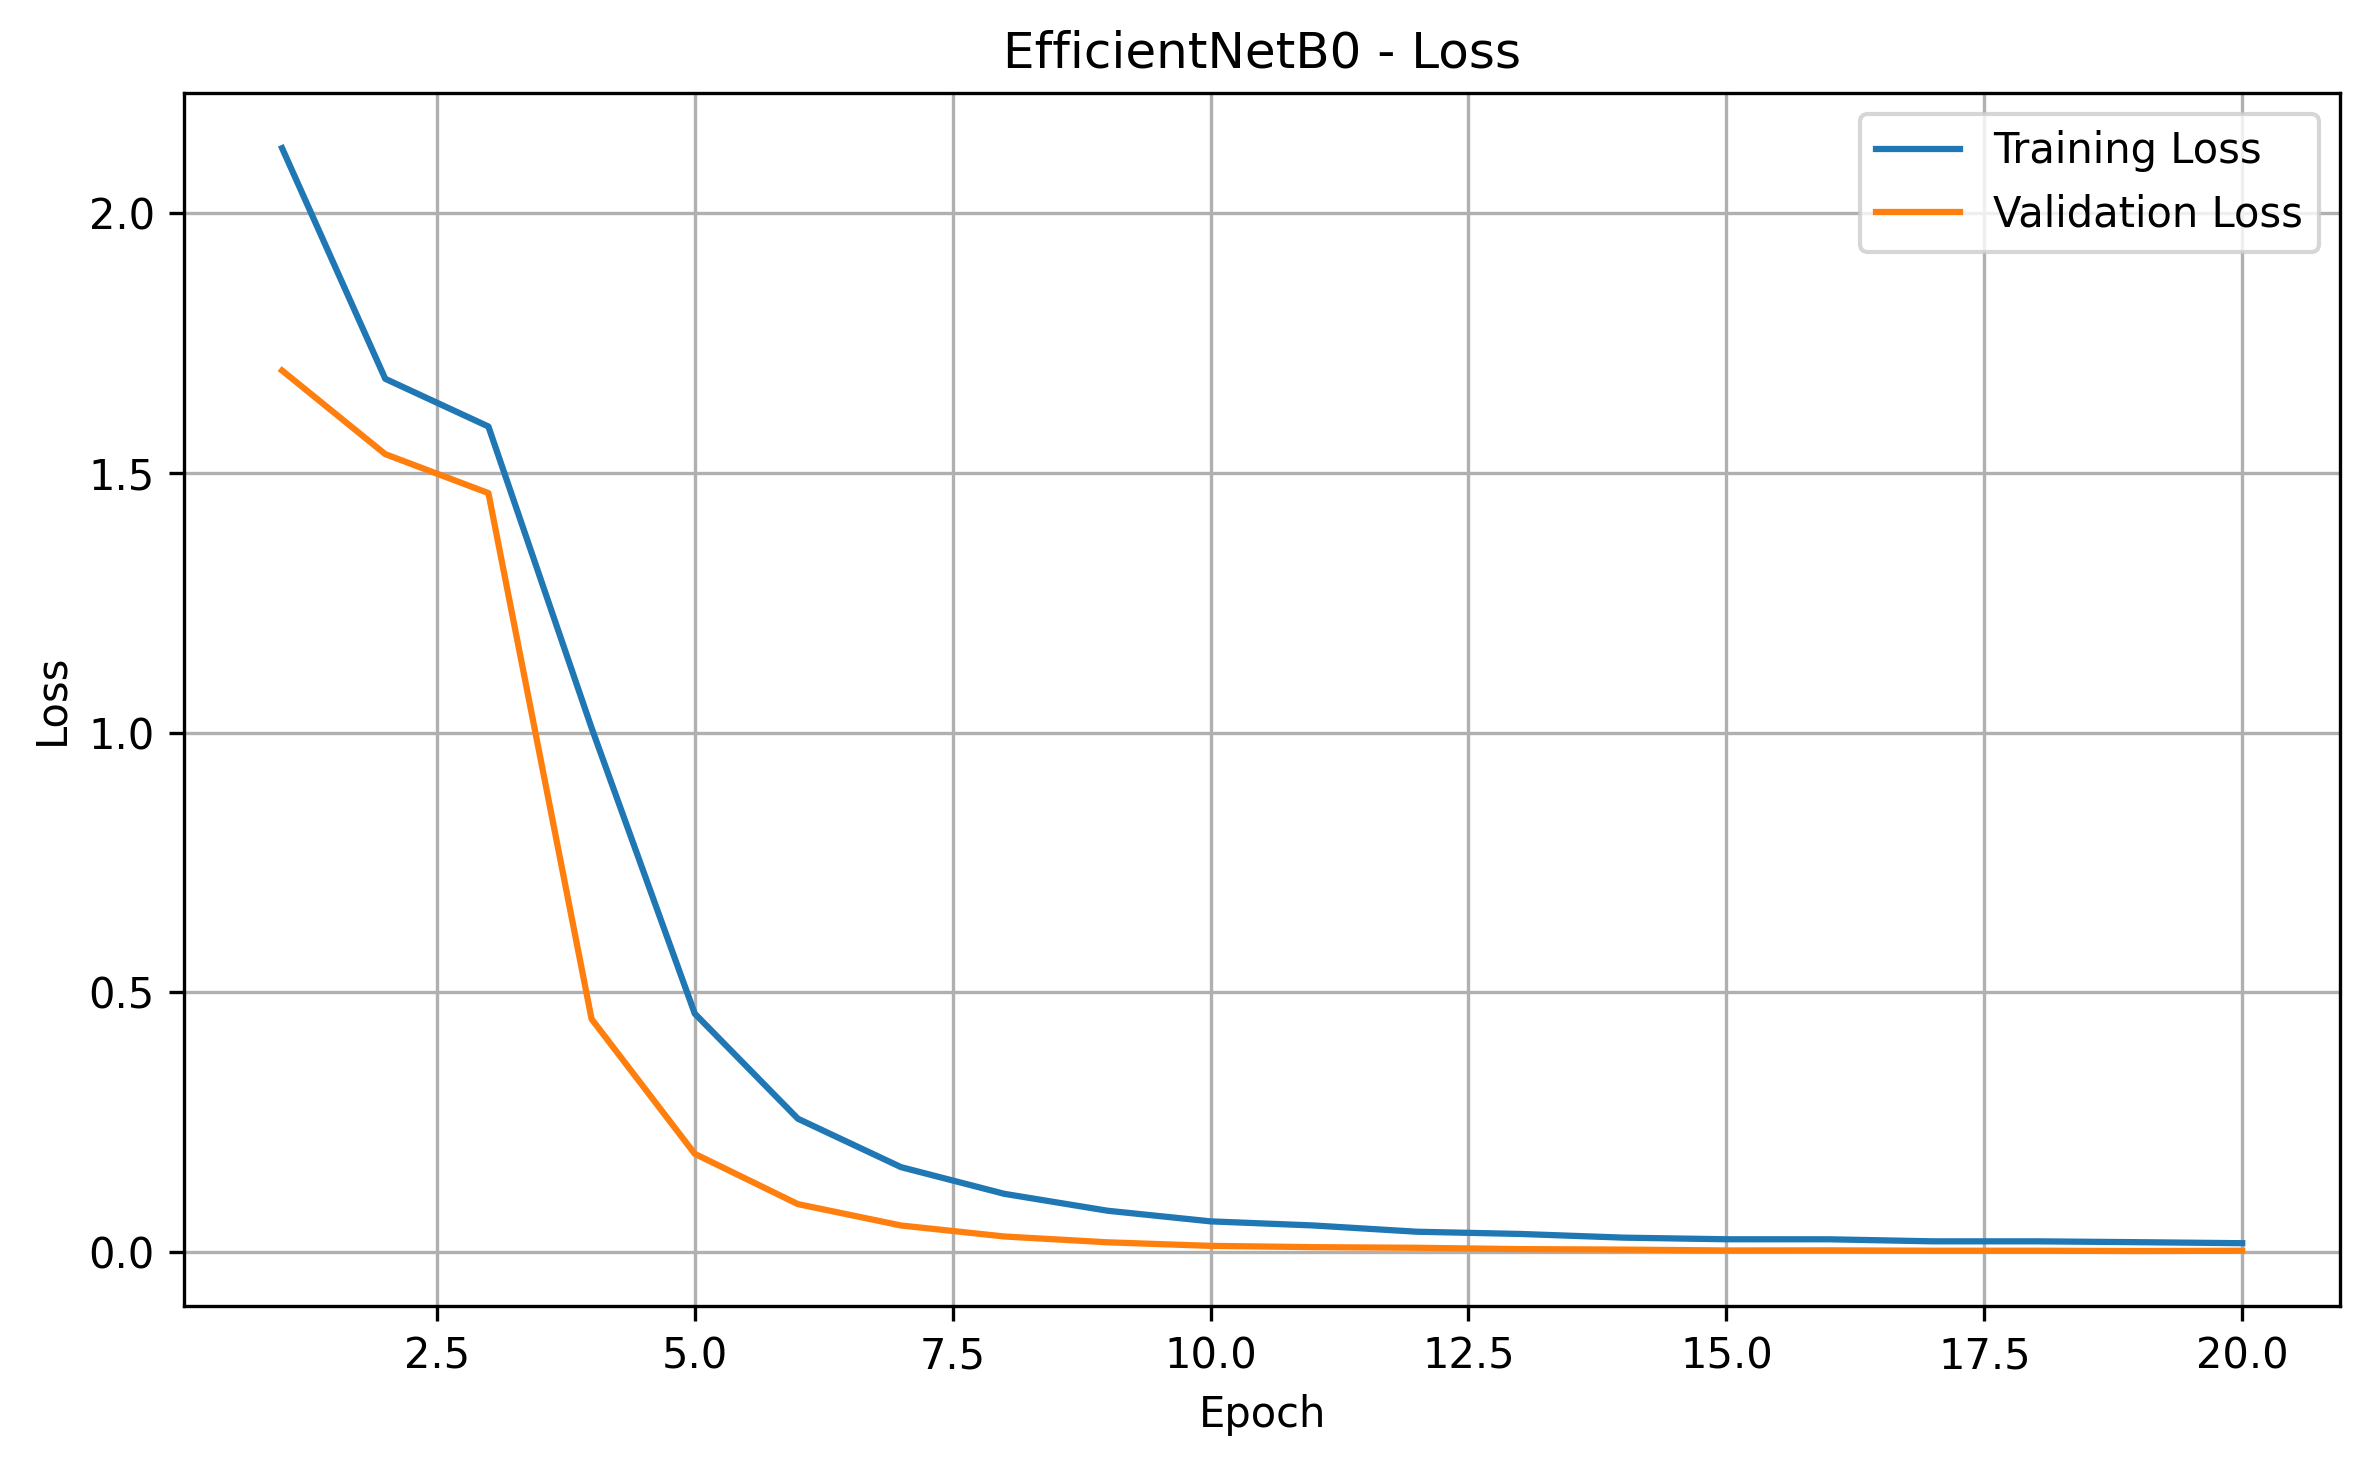
\includegraphics[width=\textwidth]{figures/efficientnetb0_loss.png}
    \caption{EfficientNet-B0}
\end{subfigure}
\caption{Training and validation loss during fine-tuning (backbone unfrozen after epoch 3).}
\label{fig:sotaloss}
\end{figure}

Table~\ref{tab:sota} summarises both models and Figure~\ref{fig:sotaloss} shows their training.
With only the head trained, validation accuracy stalls at 58\% (MobileNetV2) and 56\% (EfficientNet-B0): ImageNet
features alone do not separate $64 \times 64$ traffic signs well, because these images look very different from
ImageNet photographs and the backbone's final feature map is only $2 \times 2$. As soon as the whole network is
unfrozen, accuracy jumps to 93\% and 86\% after a single epoch and passes 99\% by epoch 7--8. Both models reach
near-perfect test accuracy and show no overfitting.

% ==========================================
\section{Final Comparison and Trade-off Discussion}
\label{sec:final}
% ==========================================

\subsection{Results}

Table~\ref{tab:final} compares the custom resource-constrained model (Model B) with the fine-tuned SOTA models;
Model A is included as a reference. To reflect an edge device more closely than a GPU, each architecture was also
timed on the CPU with \textbf{one thread and one image at a time} (median of 200 runs). The estimated 8-bit size
assumes one byte per parameter.

\begin{table}[H]
\centering
\caption{Accuracy, memory footprint and computational cost of all models.}
\label{tab:final}
\begin{tabular}{lrrrr}
\toprule
\textbf{Metric} & \textbf{Model A} & \textbf{Model B} & \textbf{MobileNetV2} & \textbf{EfficientNet-B0} \\
\midrule
\multicolumn{5}{l}{\emph{Accuracy}} \\
Test accuracy (\%)              & 98.97 & 97.00 & 100.00 & 99.82 \\
Macro precision (\%)            & 98.74 & 97.49 & 100.00 & 99.87 \\
Macro recall (\%)               & 99.17 & 97.36 & 100.00 & 99.91 \\
\midrule
\multicolumn{5}{l}{\emph{Memory footprint}} \\
Parameters                      & 45,643 & 25,526 & 2,278,955 & 4,062,631 \\
Model size on disk (MB)         & 0.179  & 0.103  & 8.93      & 15.79 \\
Estimated 8-bit size (MB)       & 0.044  & 0.024  & 2.17      & 3.87 \\
\midrule
\multicolumn{5}{l}{\emph{Computational cost}} \\
MACs per image (M)              & 9.46   & 1.42   & 24.50     & 32.02 \\
CPU latency, 1 thread (ms)      & 1.52   & 1.61   & 6.94      & 10.35 \\
GPU inference (ms/image)        & 0.36   & 0.34   & 0.60      & 0.67 \\
Training time per epoch (s)     & 41.0   & 44.2   & 55.8      & 70.1 \\
\bottomrule
\end{tabular}
\end{table}

\begin{table}[H]
\centering
\caption{Cost of each SOTA model relative to Model B, and the accuracy it gains.}
\label{tab:ratio}
\begin{tabular}{lrrrrr}
\toprule
\textbf{Model} & \textbf{Parameters} & \textbf{Size} & \textbf{MACs} & \textbf{CPU latency} & \textbf{Accuracy} \\
\midrule
MobileNetV2      & $89\times$  & $87\times$  & $17\times$ & $4.3\times$ & $+3.00$ pts \\
EfficientNet-B0  & $159\times$ & $153\times$ & $23\times$ & $6.4\times$ & $+2.83$ pts \\
\bottomrule
\end{tabular}
\end{table}

\begin{figure}[H]
\centering
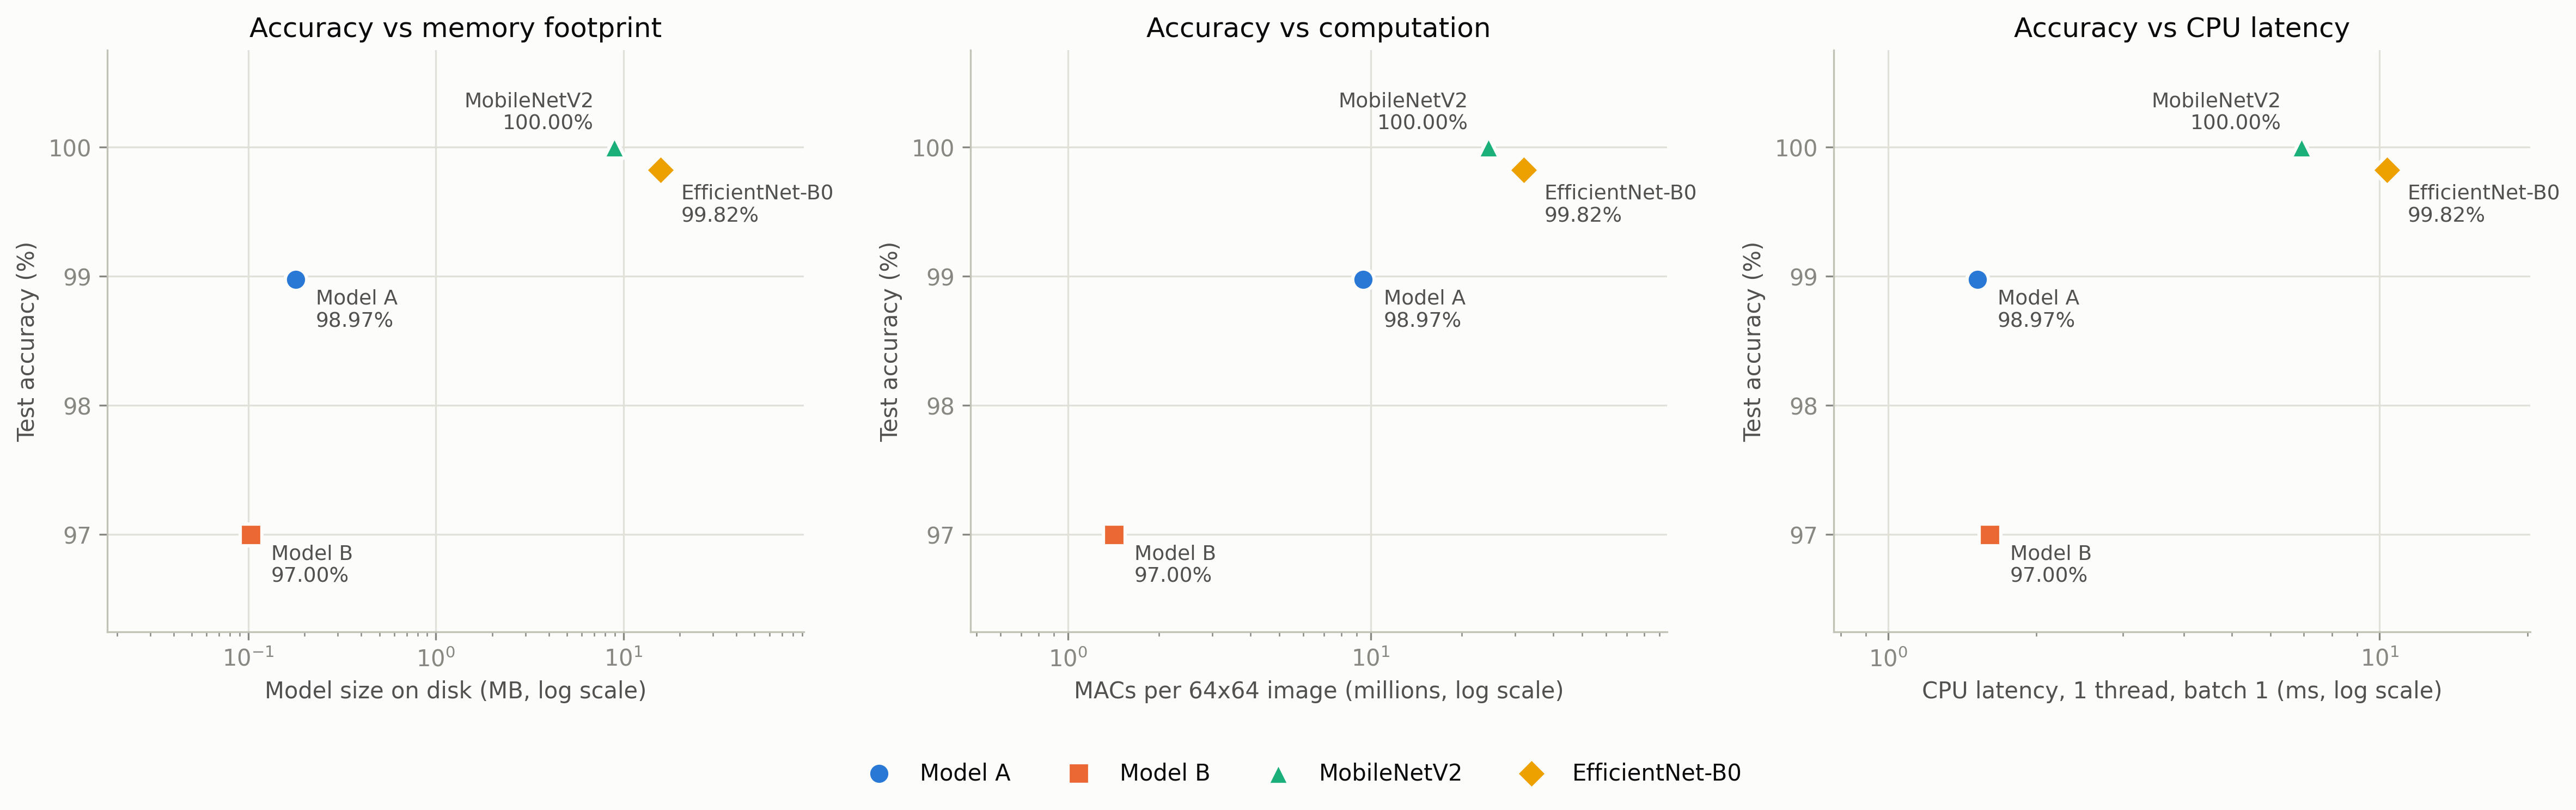
\includegraphics[width=\textwidth]{figures/final_tradeoffs.png}
\caption{Test accuracy against model size, MACs and single-thread CPU latency (logarithmic x-axes). Up and to the
left is better.}
\label{fig:tradeoffs}
\end{figure}

\begin{table}[H]
\centering
\caption{Recall (\%) on the eight classes where Model B is weakest.}
\label{tab:classes}
\resizebox{\textwidth}{!}{%
\begin{tabular}{llrrrrr}
\toprule
\textbf{Class} & \textbf{Sign} & \textbf{Test images} & \textbf{Model A} & \textbf{Model B} & \textbf{MobileNetV2} & \textbf{EfficientNet-B0} \\
\midrule
41 & End of no passing    & 35  & 94.29  & 82.86 & 100.00 & 100.00 \\
2  & Speed limit 50       & 233 & 99.14  & 88.84 & 100.00 & 98.71 \\
5  & Speed limit 80       & 209 & 98.56  & 89.95 & 100.00 & 99.52 \\
3  & Speed limit 60       & 148 & 97.97  & 92.57 & 100.00 & 100.00 \\
23 & Slippery road        & 44  & 100.00 & 93.18 & 100.00 & 100.00 \\
7  & Speed limit 100      & 155 & 98.06  & 94.19 & 100.00 & 100.00 \\
0  & Speed limit 20       & 19  & 100.00 & 94.74 & 100.00 & 100.00 \\
29 & Bicycles crossing    & 21  & 100.00 & 95.24 & 100.00 & 100.00 \\
\bottomrule
\end{tabular}}
\end{table}

\subsection{Discussion}

Table~\ref{tab:ratio} expresses each SOTA model's cost as a multiple of Model B's, and Figure~\ref{fig:tradeoffs}
places all four models on the accuracy--memory--computation trade-off.

\textbf{Accuracy.} The pretrained models are about 3 percentage points more accurate than Model B (100.00\% and
99.82\% vs 97.00\%), and the gain is concentrated on the fine-grained classes where Model B struggles
(Table~\ref{tab:classes}): MobileNetV2 recognises every speed-limit sign correctly, while Model B confuses signs that
differ only in their digits. ImageNet pretraining gives the large models rich features for edges, strokes and
shapes, which a 25,526-parameter network trained from scratch on 18,648 images cannot fully learn. Pretraining also
speeds up learning: the SOTA models pass 99\% validation accuracy by epoch 7--8, a level Model B never reaches
(Figure~\ref{fig:valacc}).

\textbf{Memory footprint.} This is where Model B wins decisively. At 0.10\,MB in 32-bit floating point, or about
25\,KB in 8-bit form, it fits comfortably in the flash and RAM of typical microcontrollers, which have a few hundred
kilobytes to a few megabytes. MobileNetV2 and EfficientNet-B0 are 87$\times$ and 153$\times$ larger and still need
2.2--3.9\,MB after 8-bit quantisation, which rules them out for most microcontrollers but is acceptable on a
Raspberry Pi-class device.

\textbf{Computational cost.} Model B needs 17--23$\times$ fewer MACs, and on a single CPU thread it is 4.3--6.4$\times$
faster than the SOTA models; this matters directly for battery life and frame rate on an edge device. The latency
ratio is smaller than the MAC ratio because these small models are partly limited by per-layer overhead rather than
arithmetic. The same effect explains why Model B is not faster than Model A on this desktop CPU and GPU despite 85\%
fewer MACs. EfficientNet-B0 is the least efficient model here: it is larger, slower and slightly less accurate than
MobileNetV2, because its design was tuned for $224 \times 224$ inputs and its SiLU activations and
squeeze-and-excitation gates require exponentials.

\begin{figure}[H]
\centering
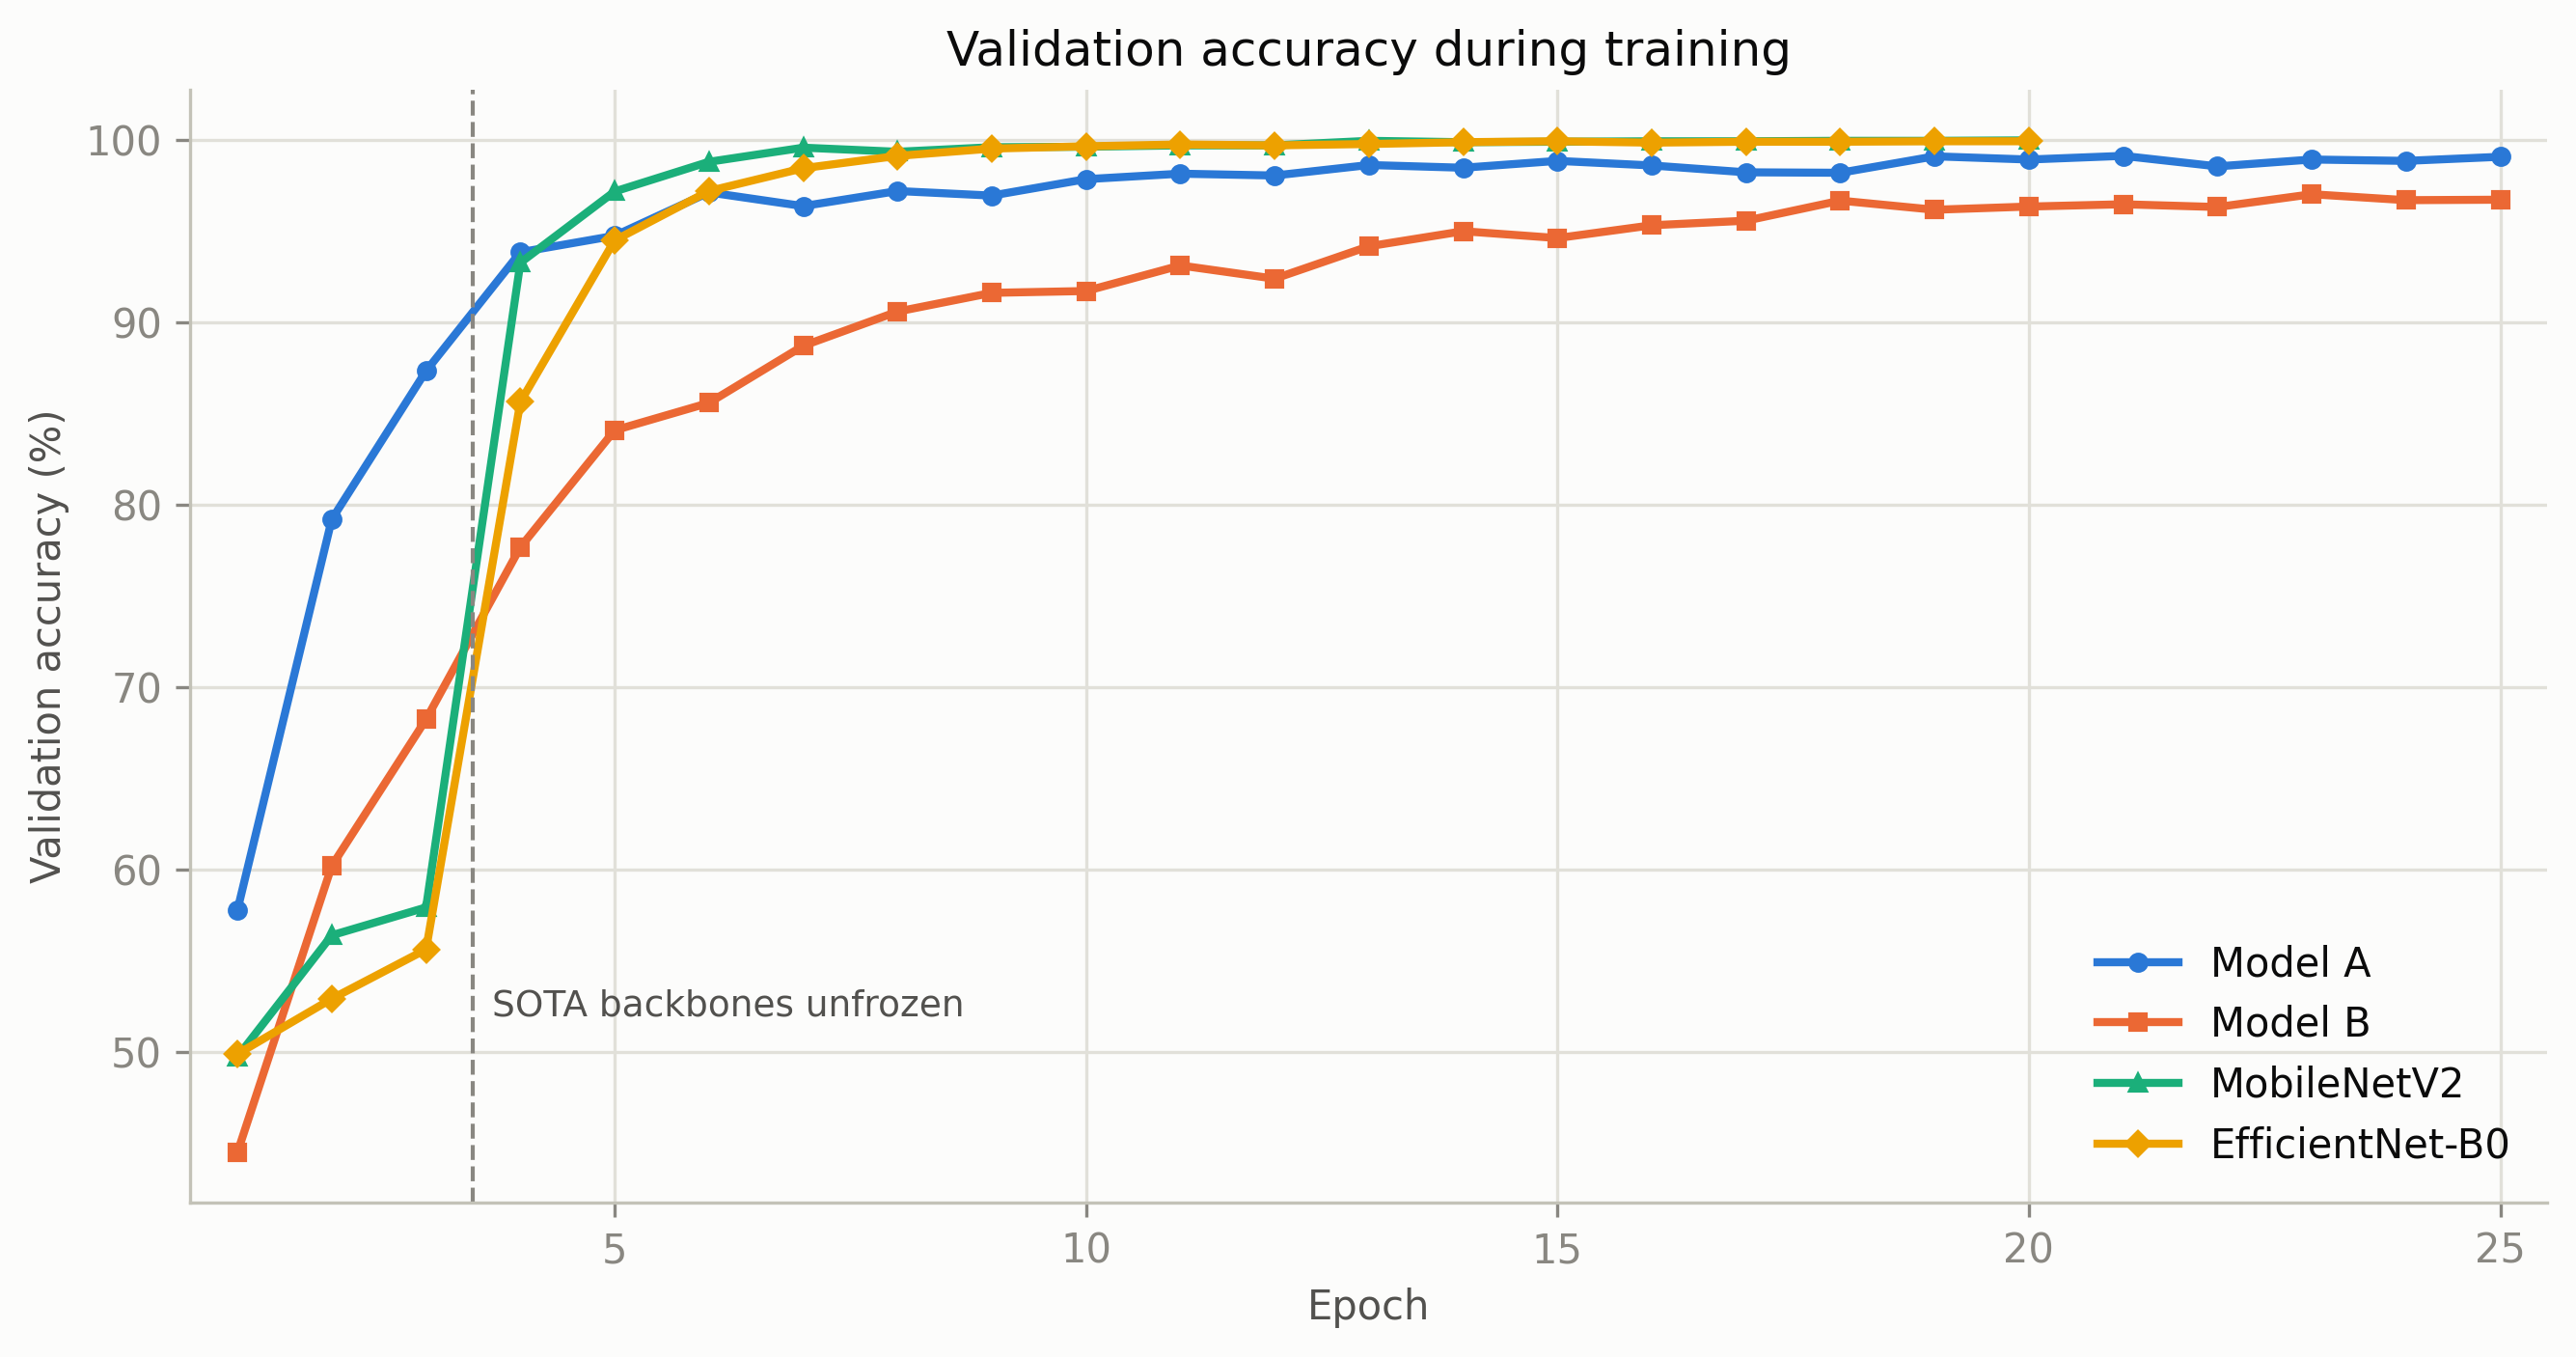
\includegraphics[width=0.7\textwidth]{figures/final_validation_accuracy.png}
\caption{Validation accuracy per epoch for all four models. The pretrained models are unfrozen after epoch 3.}
\label{fig:valacc}
\end{figure}

\textbf{Custom sub-100k model: advantages and limitations.}
\begin{itemize}
    \item[+] Tiny memory footprint (25\,KB in 8-bit form) and very low compute; deployable on microcontrollers.
    \item[+] Uses only operations that are cheap and widely supported on edge hardware (convolution, ReLU, max-pooling).
    \item[+] No dependence on large pretrained weights or a 224-pixel input; the architecture is fully under control
          and can be shaped for a specific device.
    \item[--] Lower accuracy on fine-grained classes, slower convergence, and a design that needs manual exploration.
    \item[--] Its theoretical savings only become real speed with optimised depthwise kernels on the target hardware.
\end{itemize}

\textbf{Pretrained lightweight model: advantages and limitations.}
\begin{itemize}
    \item[+] Highest accuracy and fastest convergence thanks to transfer learning; little architecture design needed.
    \item[--] 2--4\,MB even when quantised, 17--23$\times$ the MACs and 4--6$\times$ the latency of Model B; too large
          for most microcontrollers.
    \item[--] Designed for $224 \times 224$ inputs; at $64 \times 64$ much of their capacity is unused.
\end{itemize}

\textbf{Recommendation.} For a microcontroller-class device, Model B offers the best balance: 97\% accuracy within
about 25\,KB and 1.4\,M MACs per image. If the device has megabytes of memory (e.g.\ a Raspberry Pi) and the highest
accuracy is required, MobileNetV2 is the better choice: it is more accurate, smaller and faster than EfficientNet-B0.

\subsection{Limitations}

\begin{itemize}
    \item \textbf{Optimistic test accuracy.} GTSRB's training images come in \emph{tracks} of about 30 consecutive
          frames of the same physical sign. Because the split was random by image, every one of the 883 sign tracks in
          the test set also has frames in the training set. Test images are therefore very similar to training images,
          which inflates all accuracies; the 100\% of MobileNetV2 should be read in this light. A track-wise split, or
          the official GTSRB test set, would give a more realistic estimate of accuracy on unseen signs. The comparison
          between models remains fair, because all of them use the same split.
    \item \textbf{Timing on desktop hardware.} Latency was measured on a desktop CPU and GPU with 32-bit floating point.
          Real edge latency depends on the device, the inference library and 8-bit quantisation, which were not
          evaluated.
    \item \textbf{Single run.} Each model was trained once with a fixed seed; small accuracy differences (e.g.\ between
          the two SOTA models) are within run-to-run variation.
\end{itemize}

% ==========================================
\section{Conclusion}
% ==========================================

Two custom CNNs and two pretrained lightweight networks were trained and compared for $64 \times 64$ traffic-sign
classification. Replacing standard convolutions with depthwise separable convolutions cut parameters by 44\% and MACs
by 85\% (Model B: 25,526 parameters) at a cost of 2 percentage points of test accuracy (97.00\% vs 98.97\%). Adam with
$\eta = 0.001$ trained fastest and most stably; momentum accelerates SGD but overshoots when $\beta$ is too large.
Fine-tuned MobileNetV2 and EfficientNet-B0 reached 100.00\% and 99.82\% test accuracy, but are 87--153$\times$ larger
and need 17--23$\times$ more computation than Model B. For memory-constrained edge devices, a carefully designed
sub-100k-parameter model offers a far better balance of accuracy, memory and computation, while pretrained models
are preferable when memory is not the limiting factor. Fewer MACs, however, only become faster inference with
hardware and libraries optimised for depthwise convolutions.

% ==========================================
\begin{thebibliography}{9}
% ==========================================

\bibitem{gtsrb}
J.~Stallkamp, M.~Schlipsing, J.~Salmen and C.~Igel, ``Man vs.\ computer: Benchmarking machine learning algorithms
for traffic sign recognition,'' \emph{Neural Networks}, vol.~32, pp.~323--332, 2012.

\bibitem{mobilenetv1}
A.~G.~Howard \emph{et al.}, ``MobileNets: Efficient convolutional neural networks for mobile vision applications,''
arXiv:1704.04861, 2017.

\bibitem{mobilenetv2}
M.~Sandler, A.~Howard, M.~Zhu, A.~Zhmoginov and L.-C.~Chen, ``MobileNetV2: Inverted residuals and linear
bottlenecks,'' in \emph{Proc.\ IEEE CVPR}, 2018, pp.~4510--4520.

\bibitem{efficientnet}
M.~Tan and Q.~V.~Le, ``EfficientNet: Rethinking model scaling for convolutional neural networks,'' in
\emph{Proc.\ ICML}, 2019, pp.~6105--6114.

\bibitem{adam}
D.~P.~Kingma and J.~Ba, ``Adam: A method for stochastic optimization,'' in \emph{Proc.\ ICLR}, 2015.

\end{thebibliography}

\end{document}
